\documentclass[11pt]{article}

\usepackage[margin=1in]{geometry}
\usepackage{amsmath,amssymb,amsthm}
\usepackage{graphicx}
\usepackage{booktabs}
\usepackage{array}
\usepackage{siunitx}
\usepackage[hidelinks]{hyperref}

% Figures are committed copies of the campaign's generated products, so this
% note compiles from a clean clone. ../results/ is the live (git-ignored)
% output directory and is searched second, so a fresh campaign run is picked
% up automatically by anyone who has one.
\graphicspath{{figs/}{../results/}}

\newtheorem{theorem}{Theorem}
\newtheorem{proposition}{Proposition}

\newcommand{\rvec}{\mathbf{r}}
\newcommand{\vvec}{\mathbf{v}}
\newcommand{\Tvec}{\mathbf{T}}
\newcommand{\uvec}{\mathbf{u}}
\newcommand{\gvec}{\mathbf{g}}
\newcommand{\lamv}{\boldsymbol{\lambda}_v}
\newcommand{\lamr}{\boldsymbol{\lambda}_r}
\newcommand{\Tmin}{T_{\min}}
\newcommand{\Tmax}{T_{\max}}
\newcommand{\etaT}{\eta_T}

\title{Minimum-Fuel Powered-Descent Guidance for a Falcon-9-Class Booster:\\
Two Solution Routes, Five Certification Gates,\\
and What the Tracking Problem Taught Us}

\author{Michael Casey}

\date{9 August 2026}

\begin{document}
\maketitle

\begin{abstract}
This note documents a 3-DOF minimum-fuel powered-descent guidance (PDG)
campaign for a Falcon-9-class booster landing burn. The same optimal
control problem is solved two independent ways --- a free-final-time
Hermite--Simpson collocation NLP with the nonconvex thrust annulus handled
directly, and a lossless convexification solved as a sequence of fixed-time
convex subproblems under a golden-section search on $t_f$ --- and the two
answers are cross-validated through a five-gate certification layer. At the
production grid the two solvers agree on final mass to $0.43$~kg out of
$3535.4$~kg of propellant burned, and the residual is identified as the
model error of the convex formulation's Taylor mass bound rather than a
discretization gap: it does not shrink under refinement, and its sign is
the one that bound's conservatism points to. The certified optimum is
a min--max (suicide-burn) bang-bang profile, not the max--min--max structure
often quoted for Mars PDG: minimum throttle already exceeds vehicle weight,
so loitering is impossible and the fuel-optimal policy brakes as late as it
can. The guidance is closed with a phase-scheduled time-varying LQR and
Monte-Carlo tested: $99.5\%$ success over $200$ dispersed vacuum runs and
$99.0\%$ over $200$ runs with drag and wind. Most of the engineering content
of the campaign came out of the tracking problem, not the optimization: a
singular terminal boundary condition, an algebraic-Riccati pole ceiling that
no control weight can beat, altitude-indexed rather than clock-indexed
reference tracking, a guidance thrust de-rate forced by a reachability
argument, and a feed-forward reconstruction defect that silently corrupted a
certification gate by four orders of magnitude. Each is documented with the
measurement that produced it. Finally, a Phase-2 comparison with an
exponential atmosphere finds the counterintuitive result that drag
\emph{saves} $434.7$~kg of propellant while \emph{lengthening} the flight by
$0.94$~s.
\end{abstract}

\tableofcontents

\section{Problem}
\label{sec:problem}

\subsection{Dynamics and boundary conditions}

The vehicle is a point mass in a flat-Earth, constant-gravity frame with $z$
up and the landing pad at the origin. The state is
$x = [\rvec;\ \vvec;\ m] \in \mathbb{R}^7$ and the control is the thrust
vector $\Tvec \in \mathbb{R}^3$:
%
\begin{equation}
\dot{\rvec} = \vvec, \qquad
\dot{\vvec} = \gvec + \frac{\Tvec}{m} + \mathbf{a}_D, \qquad
\dot{m} = -\frac{\lVert \Tvec \rVert}{I_{sp} g_0},
\label{eq:dyn}
\end{equation}
%
with $\gvec = [0;0;-g_0]$. The drag term $\mathbf{a}_D$ is identically zero
throughout Phase~1 (Sections~\ref{sec:problem}--\ref{sec:mc}); Phase~2
(Section~\ref{sec:phase2}) switches on an exponential atmosphere,
%
\begin{equation}
\mathbf{a}_D = -\frac{1}{2}\,\rho_0 e^{-z/H}\, \frac{C_d A}{m}\,
\lVert \vvec_{rel} \rVert\, \vvec_{rel},
\qquad \vvec_{rel} = \vvec - \mathbf{w},
\label{eq:drag}
\end{equation}
%
where $\mathbf{w}$ is the wind. The guidance solves with $\mathbf{w} =
\mathbf{0}$; wind enters only as a Monte-Carlo dispersion in the truth
model (Table~\ref{tab:dispersions}), which is the honest split --- the
guidance does not know the wind.
%
Magnitudes are written as $\sqrt{\sum(\cdot)^2}$ rather than
\texttt{norm}/\texttt{abs} throughout the implementation so that the
dynamics function stays complex-step differentiable; analytic Jacobians
$A = \partial \dot{x}/\partial x$ and $B = \partial \dot{x} / \partial
\Tvec$ are returned alongside $\dot x$ and are used by the tracker of
Section~\ref{sec:tracking}.

The control set is the \emph{thrust annulus}
%
\begin{equation}
\Tmin \le \lVert \Tvec \rVert \le \Tmax ,
\label{eq:annulus}
\end{equation}
%
which is nonconvex because of its lower bound. The engine is never shut
down and never relit: a landing burn is modelled as one continuous burn
with a throttle range, which is the physical situation on this class of
vehicle and is the standard PDG formulation~\cite{acikmese2007}. A
glideslope cone $z \ge \lVert (x,y) \rVert \tan(\gamma_{gs})$ with
$\gamma_{gs} = 30^\circ$ is imposed; the thrust-pointing cone is available
but disabled ($\theta_{\max} = \infty$) for this campaign.

Boundary conditions are
$\rvec(0) = \rvec_0$, $\vvec(0) = \vvec_0$, $m(0) = m_0$, and
$\rvec(t_f) = \mathbf{0}$, $\vvec(t_f) = \vvec_f$, with $t_f$ free. The
objective is $\max\, m(t_f)$, equivalently
$\min \int_0^{t_f} \lVert \Tvec \rVert \, dt$.

The choice $\vvec_f = [0;0;-1.5]$~m/s rather than $\vvec_f = \mathbf{0}$ is
not cosmetic; it is an adjudicated design decision forced by a genuine
singularity, and Section~\ref{sec:singular} explains it.

\subsection{Parameters}

Table~\ref{tab:params} is the complete parameter set; every number in this
note follows from it plus the two solvers.

\begin{table}[htbp]
\centering
\caption{Falcon-9-class parameter set (\texttt{lib/booster\_params.m}).
Public block-5 estimates; every number is adjustable in that one file.}
\label{tab:params}
\begin{tabular}{llr@{\;}l}
\toprule
Symbol & Meaning & \multicolumn{2}{l}{Value} \\
\midrule
$m_{dry}$      & dry mass                              & $25\,600$ & kg \\
$m_0$          & mass at landing-burn ignition         & $30\,000$ & kg \\
$m_0 - m_{dry}$& usable propellant                     & $4\,400$ & kg \\
$\Tmax$        & one Merlin 1D, sea level              & $845.0$ & kN \\
$\Tmin$        & minimum throttle ($0.40\,\Tmax$)      & $338.0$ & kN \\
$\etaT$        & \emph{guidance} thrust de-rate        & $0.87$ & -- \\
$\etaT \Tmax$  & guidance thrust ceiling               & $735.15$ & kN \\
$I_{sp}$       & sea-level specific impulse            & $282$ & s \\
$I_{sp} g_0$   & effective exhaust velocity            & $2765.5$ & m/s \\
$g_0$          & standard gravity                      & $9.80665$ & m/s$^2$ \\
\midrule
$\rvec_0$      & post-entry-burn position              & \multicolumn{2}{l}{$[500;\,100;\,2000]$ m ($\lVert\rvec_0\rVert = 2064.0$ m)} \\
$\vvec_0$      & entry velocity                        & \multicolumn{2}{l}{$[-30;\,0;\,-180]$ m/s ($\lVert\vvec_0\rVert = 182.5$ m/s)} \\
$\vvec_f$      & terminal velocity target              & \multicolumn{2}{l}{$[0;\,0;\,-1.5]$ m/s (adjudicated, \S\ref{sec:singular})} \\
$\gamma_{gs}$  & glideslope minimum elevation          & $30$ & deg \\
\midrule
$N$            & Hermite--Simpson segments             & $60$ & -- \\
$N_{conv}$     & trapezoid nodes, convex solver        & $120$ & -- \\
$[t_{f,lo}, t_{f,hi}]$ & free-final-time bracket       & \multicolumn{2}{l}{$[10,\,22]$ s} \\
\midrule
$R_{pad}$      & landing accuracy requirement          & $15$ & m \\
$v_{td,\max}$  & maximum touchdown speed               & $2.0$ & m/s \\
\midrule
$\rho_0, H$    & sea-level density, scale height (Phase 2) & \multicolumn{2}{l}{$1.225$ kg/m$^3$, $8500$ m} \\
$C_d, A$       & drag coefficient, reference area (Phase 2)& \multicolumn{2}{l}{$1.0$, $10.75$ m$^2$} \\
\bottomrule
\end{tabular}
\end{table}

\subsection{The hoverslam argument}
\label{sec:hoverslam}

The single most consequential fact about this parameter set is a
thrust-to-weight inequality. At ignition mass and at dry mass,
%
\begin{equation}
m_0 g_0 = 294.20~\text{kN}, \qquad
m_{dry} g_0 = 251.05~\text{kN}, \qquad
\Tmin = 338.0~\text{kN},
\end{equation}
%
so that
%
\begin{equation}
\frac{\Tmin}{m_0 g_0} = 1.1489, \qquad
\frac{\Tmin}{m_{dry} g_0} = 1.3463, \qquad
\frac{\Tmax}{m_0 g_0} = 2.8722 .
\label{eq:tw}
\end{equation}
%
\textbf{Minimum throttle already exceeds vehicle weight at every mass on the
trajectory.} The vehicle physically cannot hover, cannot loiter, and has no
free coast: once the engine is lit, a near-vertical thrust vector always
produces a net upward (decelerating) acceleration, $1.46$~m/s$^2$ at $m_0$
and $3.40$~m/s$^2$ at $m_{dry}$. Every landing on this vehicle is a
\emph{hoverslam}: the burn must be timed so that velocity and altitude reach
zero together, because the vehicle cannot wait at the bottom for the
trajectory to catch up.

Three later results in this note are direct consequences of
Eq.~\eqref{eq:tw}: the min--max (rather than max--min--max) structure of the
optimum (\S\ref{sec:minmax}), the singularity of the $\vvec(t_f) =
\mathbf{0}$ boundary condition (\S\ref{sec:singular}), and the fact that
arriving \emph{below} the guidance's own descent-rate schedule is
unrecoverable (\S\ref{sec:altindex}).

\section{Two solution routes}
\label{sec:routes}

The campaign deliberately solves the same problem twice, by methods that
share no formulation, no discretization order, and no treatment of the
nonconvex constraint. Agreement between them is then evidence about the
\emph{problem}, not about one solver's internal consistency.

\subsection{Route A: free-final-time Hermite--Simpson collocation}
\label{sec:colloc}

Time is normalized as $t = t_f \tau$, $\tau \in [0,1]$, with $t_f$ a
decision variable. The horizon is divided into $N$ segments; the decision
vector holds the state at the $N+1$ nodes and the thrust at both nodes and
segment midpoints. Hermite--Simpson enforces, on each segment,
%
\begin{equation}
x_{k+1} - x_k - \frac{h}{6}\Big( f_k + 4 f_{k+\frac12} + f_{k+1} \Big) = 0,
\qquad
x_{k+\frac12} = \frac{x_k + x_{k+1}}{2} + \frac{h}{8}\big( f_k - f_{k+1} \big),
\label{eq:hs}
\end{equation}
%
which is the \emph{compressed} form of the third-order collocation scheme
in Kelly~\cite{kelly2017} (compressed and separated are the two alternative
formulations there; the midpoint state is eliminated here rather than
carried as a decision variable). The annulus \eqref{eq:annulus} is imposed
\emph{directly}, as written, nonconvexity and all --- this is the route that
does not need convexification to be legitimate, and it is what makes the
comparison in \S\ref{sec:crossval} meaningful. The NLP is built in CasADi
\cite{casadi2019} and solved with IPOPT \cite{ipopt2006}.

\paragraph{Why nondimensionalize.}
The formulation as literally specified --- raw SI, with $O(10^3)$~m
positions, $O(10^2)$~m/s velocities, $O(10^5)$~N thrusts and $O(10^4)$~kg
masses --- \emph{diverges} under IPOPT from a cold start even at
\texttt{maxIter}~$=6000$: the mass iterate runs past $m_0$ and $t_f$ leaves
its bracket. That is textbook-bad Hessian conditioning for a barrier method
\cite{betts2010}: a single Newton step must trade five orders of magnitude
of variable scale against each other. Nondimensionalizing the Opti variables
by characteristic scales derived from the parameter set ($L_c =
\lVert\rvec_0\rVert$, $T_c = \tfrac12 (t_{f,lo}+t_{f,hi})$, $M_c = m_0$,
with $V_c$ and $F_c$ following from $F = ma$ consistency) converges the
identical physics cold in 30--60 iterations. Every returned field is
unscaled back to SI, so the interface is unchanged, and the production solve
at $N = 60$ converges in 30 IPOPT iterations.

One consequence matters for Section~\ref{sec:certify}: the collocation
duals returned for the defect block, \verb|sol.lam_defect|, are duals of the
\emph{nondimensional} constraints. Their velocity rows (4--6) share a single
isotropic scale, so a primer-\emph{direction} check against SI thrust is
valid on the stored duals with no rescaling; cross-block identities (e.g.\
$\dot{\lamv} = -\lamr$) are off by a factor of $T_c$ unless rescaled. This
is documented at the point of extraction rather than left to be
rediscovered. The duals are taken from \verb|opti.lam_g| by explicit row
range and never from \verb|opti.dual|, following a house lesson: the latter
returns duals in a canonicalized constraint orientation whose sign depends
on how the constraint was written.

\subsection{Route B: lossless convexification}
\label{sec:convex}

The second route follows Ac\i kme\c{s}e and Ploen~\cite{acikmese2007}, whose
construction Blackmore, Ac\i kme\c{s}e and Scharf~\cite{blackmore2010} later
extended to the minimum-landing-error problem. Define
%
\begin{equation}
\uvec = \frac{\Tvec}{m}, \qquad
\sigma = \frac{\Gamma}{m}, \qquad
z = \ln m ,
\label{eq:cov}
\end{equation}
%
where $\Gamma$ is a slack thrust magnitude. Under this change of variables
the dynamics \eqref{eq:dyn} become \emph{linear} in the new state
$(\rvec,\vvec,z)$ and new control $(\uvec,\sigma)$:
%
\begin{equation}
\dot{\rvec} = \vvec, \qquad
\dot{\vvec} = \gvec + \uvec, \qquad
\dot{z} = -\alpha \sigma, \qquad \alpha \equiv \frac{1}{I_{sp} g_0},
\label{eq:linear}
\end{equation}
%
and the objective $\max m(t_f)$ becomes $\max z(t_f)$, i.e.\ $\min
\int_0^{t_f}\sigma\,dt$, which is linear.

\paragraph{The relaxation.}
The nonconvex annulus becomes the pair of constraints
%
\begin{equation}
\lVert \uvec \rVert \le \sigma, \qquad
\Tmin e^{-z} \le \sigma \le \etaT \Tmax\, e^{-z},
\label{eq:relax}
\end{equation}
%
of which the first is a second-order cone --- convex --- and the second is
still nonconvex only through $e^{-z}$. The original set is recovered exactly
when $\lVert\uvec\rVert = \sigma$ holds; the relaxation permits
$\lVert\uvec\rVert < \sigma$, which would be physically meaningless (a
vehicle throwing away mass flow without producing thrust).

\paragraph{The Taylor mass bound.}
Note carefully which half is the problem. The \emph{lower} bound
$\Tmin e^{-z} \le \sigma$ is already convex --- it is a sublevel set of the
convex function $\Tmin e^{-z} - \sigma$ --- so it needs no treatment on
convexity grounds at all. It is only the \emph{upper} bound
$\sigma \le \etaT\Tmax e^{-z}$ that is nonconvex, because it asks $\sigma$
to lie below a convex function. The construction below therefore does two
different jobs on the two bounds: it \emph{convexifies} the upper one, and
on the lower one it merely trades an exactly-convex exponential for a
quadratic, buying second-order-cone/quadratic representability (and a
solver-friendly Hessian) rather than convexity.

The remaining nonconvexity in \eqref{eq:relax} is handled by linearizing
about a \emph{maximum-thrust depletion reference}
%
\begin{equation}
z_0(t) = \ln\!\big( m_0 - \alpha\, \etaT \Tmax\, t \big),
\qquad
\delta z \equiv z - z_0 ,
\label{eq:z0}
\end{equation}
%
and imposing, with $\mu_1 = \Tmin e^{-z_0}$ and $\mu_2 = \etaT \Tmax
e^{-z_0}$,
%
\begin{equation}
\mu_1\Big(1 - \delta z + \tfrac{1}{2}\delta z^2\Big)
\;\le\; \sigma \;\le\;
\mu_2 \big(1 - \delta z\big) .
\label{eq:taylor}
\end{equation}
%
The reference is chosen as the maximum-thrust depletion for a specific
reason: no admissible trajectory can lose mass faster than $\etaT\Tmax$
allows, so $m(t) \ge m_0 - \alpha \etaT \Tmax t$ and therefore $\delta z \ge
0$ everywhere. On $\delta z \ge 0$ one has $1 - \delta z + \tfrac12 \delta
z^2 \ge e^{-\delta z}$ and $1 - \delta z \le e^{-\delta z}$, so
\eqref{eq:taylor} is a \emph{conservative} inner approximation of the true
throttle band on both sides. The upper bound is now affine in $z$ (the
nonconvexity is gone) and the lower bound is convex quadratic (it was
already convex; it is now representable), so the fixed-$t_f$ subproblem is
a genuine convex program --- second-order cone plus convex quadratic
constraints --- and by convexity any local optimum is the global
one~\cite{boyd2004}. That is the structural advantage this route buys in
exchange for the approximation in \eqref{eq:taylor}.

Conservatism has a directional consequence, which we return to in
\S\ref{sec:crossval}: the convex problem is a \emph{restriction} of the
true continuous-time problem, so its optimum is bounded above by the true
optimum. That alone does not order the two \emph{computed} answers --- the
collocation solver returns a discretized local optimum, which is likewise
an approximation of the true optimum from an unknown side --- but it does
give a direction the measured residual can either corroborate or
contradict.

\paragraph{Tightness.}

\begin{theorem}[Lossless convexification, \cite{acikmese2007,acikmese2011}]
\label{thm:lossless}
Let $(\rvec^\ast, \vvec^\ast, z^\ast, \uvec^\ast, \sigma^\ast)$ be an
optimal solution of the relaxed problem \eqref{eq:linear}--\eqref{eq:relax}.
Then $\lVert \uvec^\ast(t)\rVert = \sigma^\ast(t)$ for almost every
$t \in [0,t_f]$, so $(\rvec^\ast, \vvec^\ast, z^\ast)$ is feasible --- and
hence optimal --- for the original nonconvex problem.
\end{theorem}

\begin{proof}[Proof sketch via the maximum principle]
Form the Hamiltonian for \eqref{eq:linear} with running cost $\alpha\sigma$:
%
\begin{equation}
\mathcal{H} = \lamr\!\cdot\! \vvec
 + \lamv\!\cdot\!\big(\gvec + \uvec\big)
 - \lambda_z\, \alpha \sigma
 + \alpha \sigma .
\end{equation}
%
Take for the sketch the unconstrained-path case (glideslope inactive), so
that no state-constraint multiplier appears. The dynamics are then linear
and $\mathcal{H}$ is independent of $\rvec$ and $\vvec$ beyond the terms
shown, so the costate equations are
%
\begin{equation}
\dot{\lamr} = -\frac{\partial \mathcal{H}}{\partial \rvec} = \mathbf{0},
\qquad
\dot{\lamv} = -\frac{\partial \mathcal{H}}{\partial \vvec} = -\lamr,
\qquad
\dot{\lambda}_z = 0 .
\end{equation}
%
(The third equation is where the sketch is loosest: with an active
glideslope or throttle-bound multiplier, $\lambda_z$ acquires the
corresponding state-dependent term. It does not affect the argument below,
which turns only on $\lamv$.)
Hence $\lamr$ is constant and $\lamv(t) = \lamv(0) - \lamr t$ is
\emph{affine} in $t$. Pontryagin's minimum principle requires
$\uvec^\ast(t)$ to minimize $\lamv\!\cdot\!\uvec$ over the ball
$\lVert\uvec\rVert \le \sigma^\ast(t)$, whose unique minimizer whenever
$\lamv(t) \ne \mathbf{0}$ is
%
\begin{equation}
\uvec^\ast(t) = -\,\sigma^\ast(t)\, \frac{\lamv(t)}{\lVert \lamv(t)\rVert},
\qquad\text{so}\qquad
\lVert \uvec^\ast(t)\rVert = \sigma^\ast(t).
\label{eq:primer}
\end{equation}
%
It remains to exclude $\lamv \equiv \mathbf{0}$ on a set of positive
measure. Since $\lamv$ is affine, vanishing on a set of positive measure
forces $\lamr = \mathbf{0}$ and $\lamv \equiv \mathbf{0}$ identically. This
degenerate branch is \emph{not} closed off by transversality here: with
$\rvec(t_f)$ and $\vvec(t_f)$ both fully constrained, transversality leaves
$\lamr(t_f)$ and $\lamv(t_f)$ free, and the nontriviality condition is
satisfied by $(\lambda_z, \lambda_0)$ alone. Excluding it is exactly the
technical work done in the literature, under a controllability (normality)
assumption on the linearized system --- see Ac\i kme\c{s}e and
Ploen~\cite{acikmese2007} and, for the general class, Ac\i kme\c{s}e and
Blackmore~\cite{acikmese2011}, whose Theorem is what makes the statement
above a theorem rather than a heuristic. Granting it, $\lamv$ vanishes at
most at isolated instants and \eqref{eq:primer} holds a.e.
\end{proof}

Equation \eqref{eq:primer} is Lawden's primer-vector law
\cite{lawden1963} in the convexified variables: \emph{thrust points along
the velocity-costate direction, and its magnitude is bang--bang}.

\paragraph{A sign convention, stated once.}
Equation~\eqref{eq:primer} carries a minus sign because $\lamv$ there is
the PMP costate of the \emph{minimum} principle. Gate G5 of
\S\ref{sec:certify} instead measures alignment against
$+\lamv/\lVert\lamv\rVert$, because it reads $\lamv$ from the NLP's
\emph{defect duals} (\S\ref{sec:colloc}), whose sign is fixed by how the
defect constraint was written, not by the PMP convention --- the two differ
by exactly one overall sign. This was resolved empirically and once: the
literal minus-sign form measured $179.7$--$179.9^\circ$ at every grid, the
signature of a convention flip rather than a misaligned solution, and the
sign was flipped a single time at the point of extraction. No absolute
value was introduced anywhere, so a genuine $180^\circ$ regression would
still be caught. Wherever this note says ``the maximizing direction is
$+\lamv/\lVert\lamv\rVert$'' (\S\ref{sec:certify}, \S\ref{sec:phase2}) it
means in the defect-dual convention; \eqref{eq:primer} is the same
statement in the PMP convention.

We do not
take Theorem~\ref{thm:lossless} on faith --- gate G4 of
\S\ref{sec:certify} \emph{measures} $\max_t\, \big|\lVert\uvec\rVert -
\sigma\big|$ on the computed solution, and gate G5 measures the alignment
angle in \eqref{eq:primer} on the \emph{collocation} solver's duals.

\paragraph{Free final time.}
The convex machinery requires $t_f$ fixed. The outer loop is a
golden-section search maximizing $m(t_f)$ over $[t_{f,lo}, t_{f,hi}] =
[10,22]$~s, which is legitimate because $m(t_f)$ is unimodal on this
bracket (verified by a direct sweep). The flagship search evaluated 14
fixed-$t_f$ convex subproblems. Two practical adaptations were forced by
measurement and are recorded in the solver: (i) the subproblem is also
nondimensionalized in $\rvec$ and $\vvec$ only ($L_c = \lVert\rvec_0\rVert$,
$V_c = L_c/t_f$; $z$, $\uvec$, $\sigma$ are already $O(1)$--$O(30)$),
without which IPOPT returned \texttt{Infeasible\_Problem\_Detected} at some
$t_f$ and ``success'' with a lossless gap of up to $\sim 500$ at others,
\emph{on a convex problem}; and (ii) probes are classified
tightness-first rather than status-string-first --- one probe converged
deterministically to \texttt{Solved\_To\_Acceptable\_Level} with an
excellent gap, and rejecting it on the status string alone cost the golden
search 52~kg of final mass.

The upper bracket $t_{f,hi}$ was narrowed from $50$~s to $22$~s after a
dedicated sweep found a reproducible infeasibility wall near $t_f \approx
27$~s --- loitering that long burns past $m_{dry}$, since by
\eqref{eq:tw} there is no free coast --- with a numerically marginal band
just below it in which the \emph{identical} call measured a tight gap
($6.5\times10^{-5}$) in one process and an untight one ($0.448$) in another.
That is IPOPT/BLAS threading sensitivity, not a feasibility change, but the
old bracket's golden-ratio probe points landed squarely in it.

\subsection{Cross-validation, and what the residual is}
\label{sec:crossval}

At the production grid ($N = 60$, $N_{conv} = 120$):

\begin{table}[htbp]
\centering
\caption{The two routes at the flagship configuration.}
\label{tab:crossval}
\begin{tabular}{lrrr}
\toprule
& Route A (collocation) & Route B (convexification) & difference \\
\midrule
$t_f$ [s]        & $16.595192$  & $16.598601$ & $3.41\times10^{-3}$ \\
$m(t_f)$ [kg]    & $26464.589$  & $26464.161$ & $0.428$ \\
propellant [kg]  & $3535.411$   & $3535.839$  & $0.428$ \\
\bottomrule
\end{tabular}
\end{table}

The two solvers agree on final time to $3.4$~ms and on final mass to
$0.43$~kg out of $3535.4$~kg burned --- one part in $8\,300$ of the
propellant, or $1.6\times10^{-5}$ of the vehicle mass.

The honest framing of the residual matters more than its size.
Early in the campaign the cross-method gate was specified at $0.1$~kg and
the measured gap was $\sim 0.70$~kg, so the natural first move was to
refine until it closed. It does not close. A dedicated sweep at
\emph{fixed} $t_f$ (removing the golden search's own $t_f$-selection noise)
across $N_{conv} \in \{120, 180, 240, 300\}$ held the gap in a $0.70$--$0.74$~kg
band with no downward trend, and tightening the golden-section tolerance
from $0.05$~s to $0.01$~s did not help either. The gap is not a
discretization artifact.

It is the Taylor bound. Equation~\eqref{eq:taylor} is a conservative inner
approximation, so the convex route solves a slightly \emph{harder} problem
than the continuous-time original, and would be expected to burn slightly
\emph{more} propellant. The measurement is consistent with that and
corroborates it: $m_V(t_f) = 26464.161 < 26464.589 = m_C(t_f)$, i.e.\ the
convex route reports the larger fuel figure, which is the side the
restriction argument points to. This is corroboration, not proof --- a
rigorous ordering of the two \emph{computed} masses would additionally
require the collocation answer to be the global optimum of the
continuous-time problem (which nothing here establishes; see
\S\ref{sec:minmax}) and a bound on its own discretization error. The
magnitude, $\sim 0.02\%$ of the fuel burned, is
what that conservatism costs. On that evidence the gate threshold was
adjudicated upward to $1.0$~kg with the explicit reclassification that G3
is a \emph{measurement of a bounded, understood modelling effect}, not an
agreement tolerance the two solvers should be tuned to close. The raw
number is still reported unrounded regardless of where the threshold sits.

This is the difference between a gate and an escape hatch, and it is the
standard the rest of the campaign is held to: a relaxed threshold must
remain a measurement with headroom.

\section{Certification}
\label{sec:certify}

The certification layer (\texttt{certify/certify\_pdg.m}) exists because a
converged NLP proves less than it appears to. Its architecture is five
gates, of which the second (continuous accuracy) has two halves: G2 asks
whether the reconstructed control \emph{flies} to the right place, and G2ff
asks whether that same reconstruction is \emph{admissible} while doing it.
They share a reconstruction and a failure history, which is why they are one
gate and not two.

\paragraph{G1 --- discrete defect.}
The Hermite--Simpson defects \eqref{eq:hs} are re-evaluated in plain MATLAB
using \texttt{pdg\_dynamics}, independently of the CasADi graph the NLP was
actually solved with, and the maximum over all rows and segments is
reported. This catches a mis-built NLP, not an inaccurate one.

\paragraph{G2 --- continuous residual.}
\emph{Defect is not accuracy.} G1 only proves that the discrete constraints
were satisfied at the sample points; it says nothing about the trajectory
between them. G2 reconstructs the control as a continuous function of time,
re-integrates \eqref{eq:dyn} with \texttt{ode45} from the same initial
state, and reports the position, velocity and mass mismatch against the
NLP's own terminal state. This is the first real accuracy measurement in the
pipeline.

The reconstruction turned out to be the whole story, twice. The gate was
originally specified with a single global \texttt{pchip} spline through all
nodes and midpoints. That measured a mass residual which \emph{plateaued} at
$0.6$--$0.8$~kg for $N \ge 60$ and did not shrink out to $N = 240$ --- the
signature of a representation mismatch rather than a real continuous-time
error, because a global spline is not the control Simpson's rule is built
against. Simpson's rule assumes a \emph{separate quadratic per segment}, the
Lagrange interpolant through $(U_k, U_{k+1/2}, U_{k+1})$. Re-flying the
\emph{same saved solutions} with that reconstruction collapsed the $N=60$
mass residual from $0.7897$~kg to $1.30\times10^{-5}$~kg --- a factor of
$60\,700$ --- and did the same at $N = 240$. The floor was an artifact of
the gate's own reconstruction choice, and it had been large enough to fail a
physically accurate solution: a false negative, which is the worse failure
mode for a certification gate.

The second round came later. With the guidance de-rate of
\S\ref{sec:derate} in place, G2's \emph{position} residual failed at
$1.287$~m against a $1$~m gate. A sweep over nine $(\etaT, N)$ combinations
showed the residual ranging from $7.33\times10^{-5}$ to $1.287$~m --- the
same physics, $N=60$ versus $N=80$, moving the gate by a factor of $2000$.
The previously passing configuration had been a grid lottery ticket, not a
property. Localizing the mass error in time showed the entire residual is
generated inside \emph{one} segment: the bang-bang switch. A quadratic
through the three samples of a step is the wrong basis function. The fix
reconstructs $\lVert\Tvec\rVert$ on a transition segment as a \emph{step}
between the certified bang-bang levels, placed at the instant $s$ satisfying
%
\begin{equation}
s\,\Tmin + (h - s)\,\etaT\Tmax
= \frac{h}{6}\Big( \lVert\Tvec_k\rVert + 4\lVert\Tvec_{k+1/2}\rVert
+ \lVert\Tvec_{k+1}\rVert \Big),
\label{eq:switchstep}
\end{equation}
%
so that the step's integral \emph{equals the segment's own Simpson
quadrature}. The direction is left untouched (the primer direction is
continuous through a switch; only the magnitude steps), and both levels are
annulus samples, so feasibility is preserved by construction. After the fix
the same nine-combination sweep lands uniformly in $0.002$--$0.051$~m: the
lottery is gone, and the honest continuous accuracy of the reconstruction is
$\sim 10^{-2}$~m.

\paragraph{G2ff --- feed-forward annulus feasibility (second half of G2).}
G1 checks discrete defects; G2 checks aggregate accuracy; G5 checks the
sampled control. None of them can see a reconstruction that leaves the
annulus \emph{between} samples. Before the direction/magnitude split, the
reconstructed control dipped up to $18\%$ below $\Tmin$ over $11.7\%$ of the
flight at a coarse grid --- invisible to every gate that existed, and turned
by the closed-loop simulator's saturating clamp into a real
$+0.6$ to $1$~m open-loop altitude bias that two rounds of tracker tuning
were unknowingly fighting. G2ff densely samples the reconstruction (20
points per segment) and reports the worst fractional excursion below $\Tmin$
and above $\etaT\Tmax$. It is gated at every grid, because the fix makes a
violation impossible by construction at any resolution.

\paragraph{G3 --- cross-method agreement.}
$|\Delta m_f|$, $|\Delta t_f|$ and the $L_\infty$ position-trajectory
difference between Routes A and B. Reclassified as a measurement, per
\S\ref{sec:crossval}.

\paragraph{G4 --- losslessness.}
$\max_t \big|\lVert\uvec\rVert - \sigma\big|$ on the convex solution,
against a threshold scaled by the vehicle's own characteristic acceleration,
$10^{-4}\,\etaT\Tmax/m_0 = 2.45\times10^{-3}$~m/s$^2$. This is the numerical
check on Theorem~\ref{thm:lossless}.

\paragraph{G5 --- PMP structure.}
Two textbook necessary conditions. \emph{Bang--bang}: at least $95\%$ of the
node-and-midpoint thrust samples must lie on a bound, with at most two
interior switches, and maximum thrust must be held at touchdown.
\emph{Primer alignment}: the angle between the applied thrust direction and
$+\lamv/\lVert\lamv\rVert$, taken from the collocation duals
\verb|lam_defect| (which \S\ref{sec:colloc} established are directionally
valid unrescaled), must be under $1^\circ$.

\subsection{Flagship gate table}

The following is the verbatim gate report from
\texttt{results/booster\_run.mat}, Phase 1, at $N = 60$ / $N_{conv} = 120$
with no tolerance scaling.

{\footnotesize
\begin{verbatim}
Gate                                    value              threshold   verdict
------------------------------------------------------------------------------------
G1 max HS defect                  1.39238e-07                < 1e-06   PASS
G2 pos residual [m]                0.00884687                    < 1   PASS
G2 vel residual [m/s]             0.000298943                  < 0.1   PASS
G2 mass residual [kg]             8.23742e-06                  < 0.5   PASS
  -> G2 gate                                                           PASS
G2ff below-Tmin frac              1.72212e-16                < 1e-06   PASS
G2ff above-Tmax frac              1.58356e-16                < 1e-06   PASS
  -> G2ff gate                                                         PASS
G3 |dmf| [kg]                         0.42792                    < 1   PASS
G3 |dtf| [s]                       0.00340864                  < 0.2   PASS
G3 traj Linf [m]                     0.372616                 (info)
  -> G3 gate                                                           PASS
G4 lossless gap [m/s^2]           0.000135597        < 1e-4*TmaxG/m0   PASS
G5 bound fraction                    0.991736                >= 0.95   PASS
G5 interior switches                        1                   <= 2   PASS
G5 structure (bound+switch+max-last)                                         PASS
G5 primer angle [deg]                0.574131                    < 1   PASS
  -> G5 gate                                                           PASS
------------------------------------------------------------------------------------
ALL GATES                                                              PASS
\end{verbatim}
}

Every gate passes with margin: G1 by a factor of seven, G2's mass residual
by nearly five orders, G2ff at the level of floating-point noise, G3's
$|\Delta m_f|$ with $57\%$ of its (adjudicated) ceiling unused, G4 by a
factor of $18$, and G5's primer angle at $0.574^\circ$ against a $1^\circ$
gate. The bound fraction $0.9917$ is exactly $1$ sample of $121$ off a
bound --- one midpoint sitting inside the annulus at the switch, which is
the correct answer for a discretized step, not a defect.

\begin{figure}[htbp]
\centering
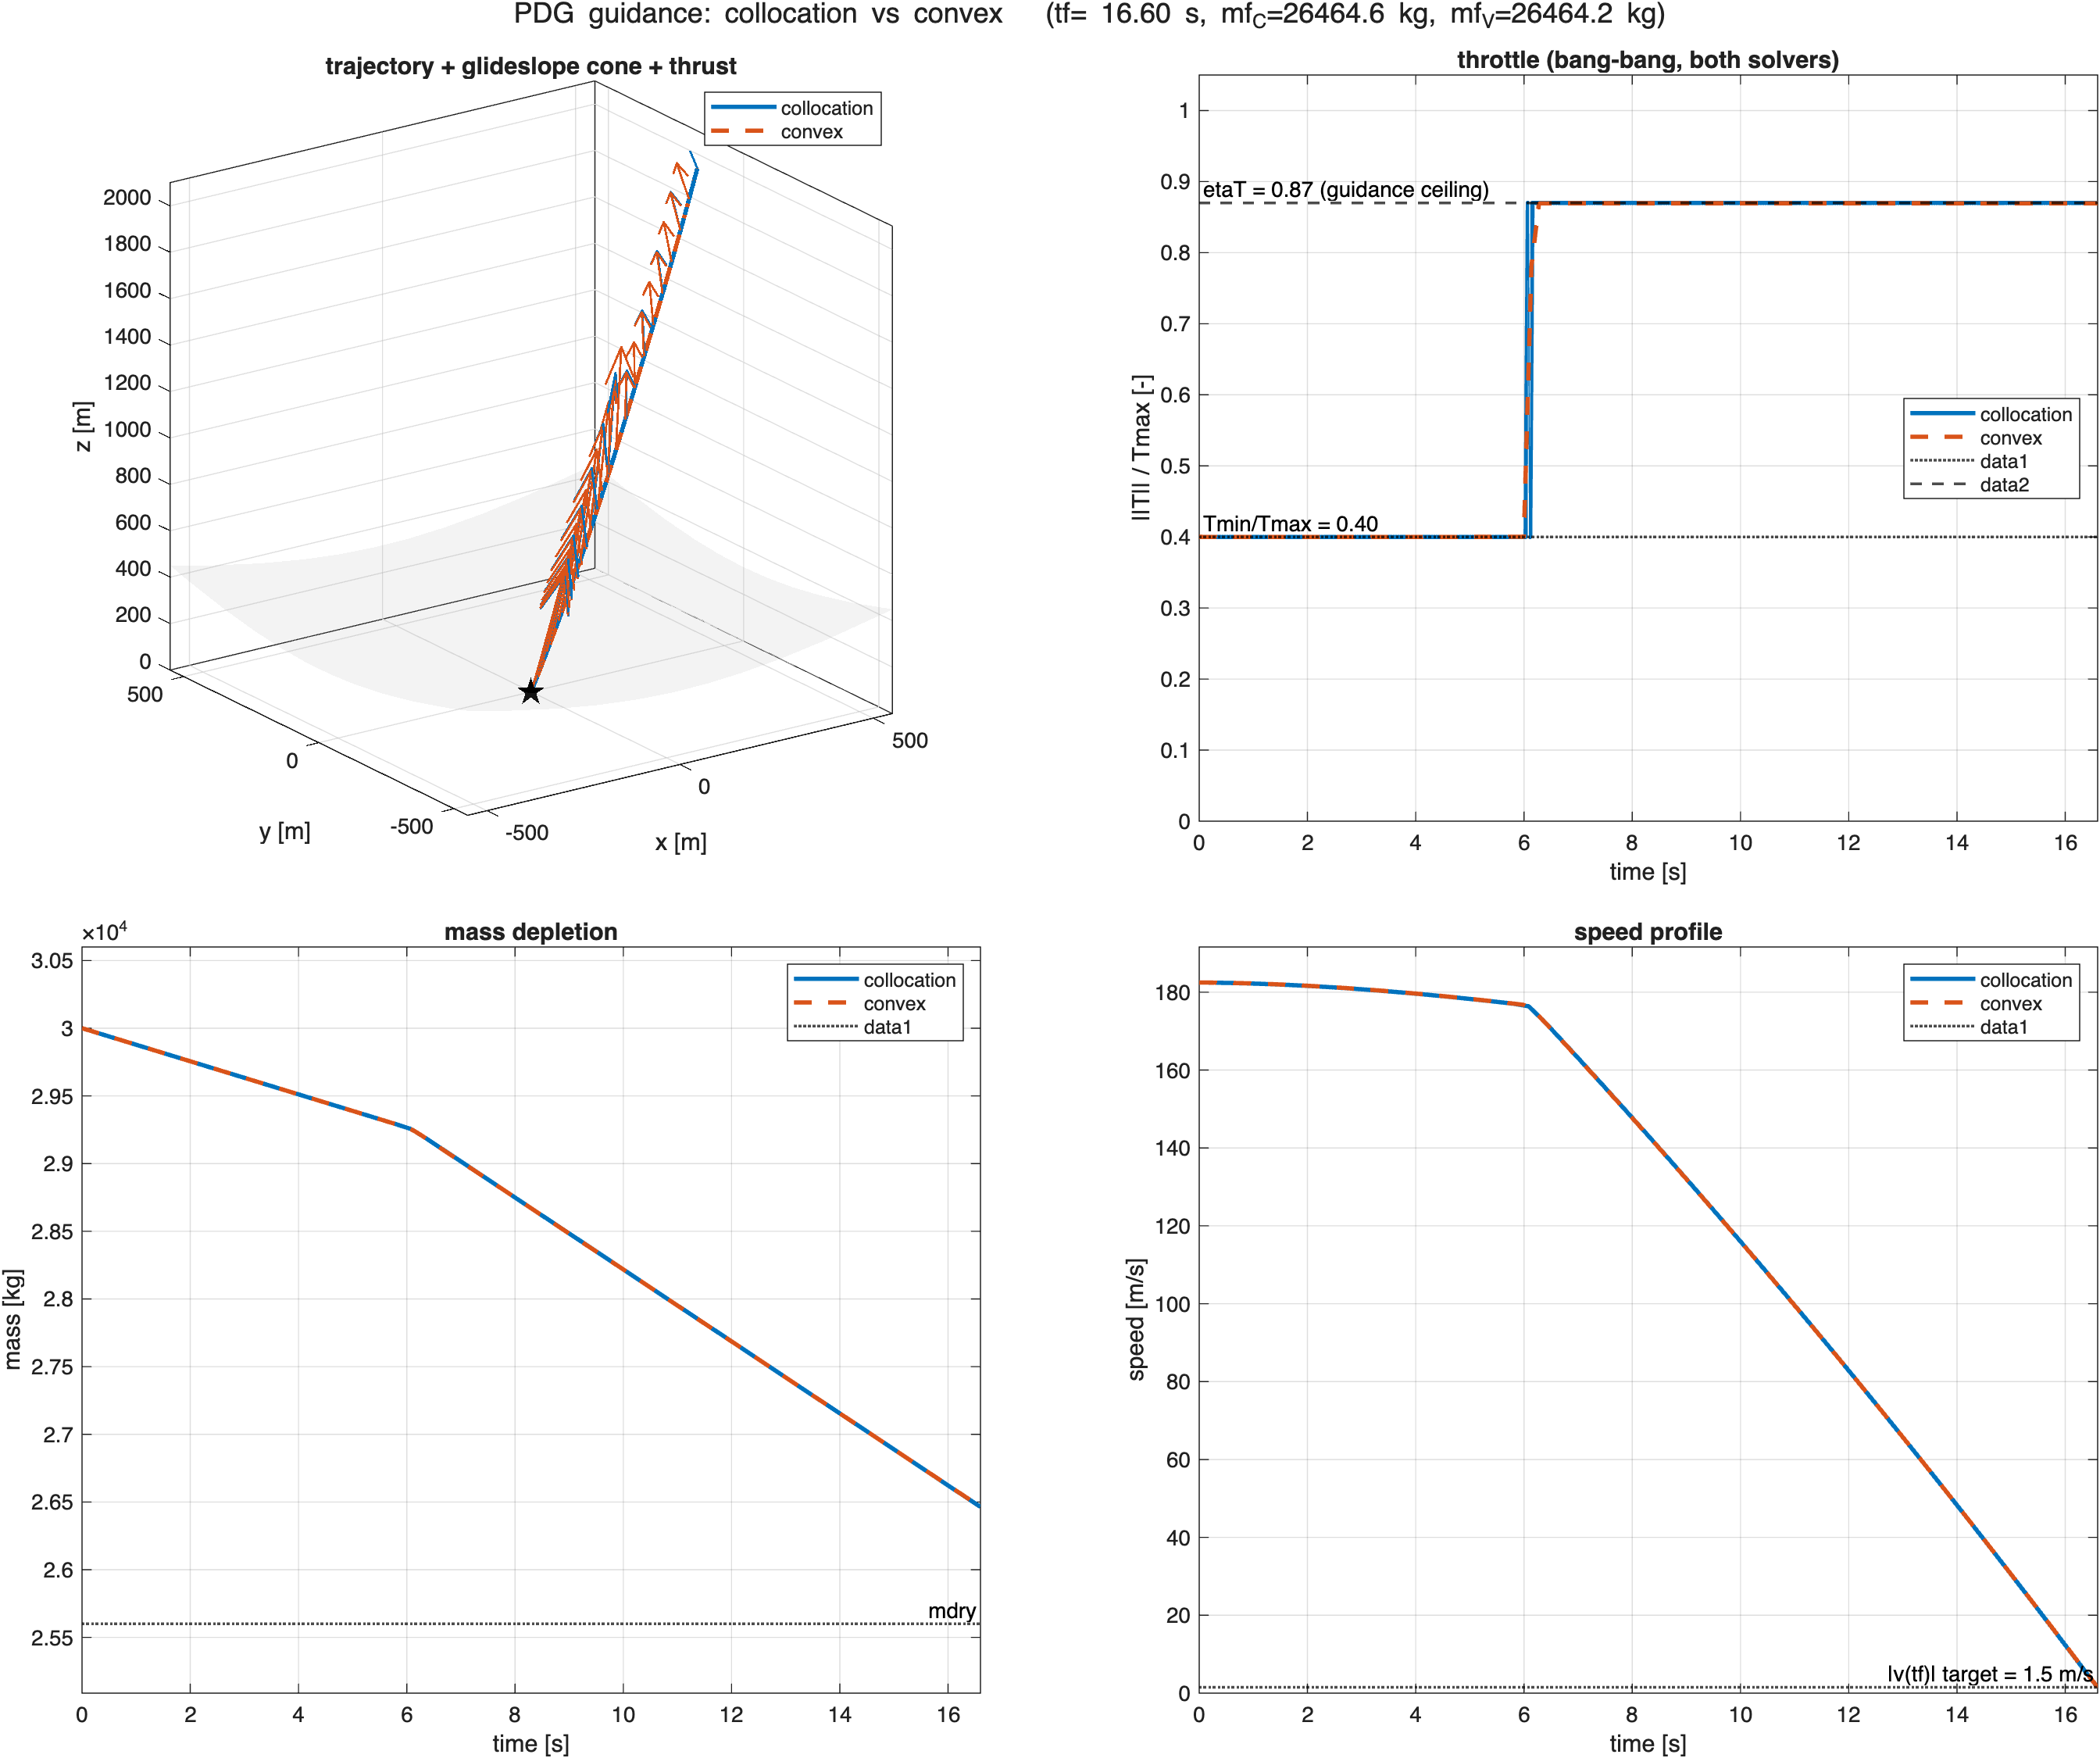
\includegraphics[width=\textwidth]{pdg_solution.png}
\caption{Flagship solution, both routes overlaid. Clockwise from top left:
three-dimensional descent trajectory with the glideslope cone; throttle
magnitude showing the single min-to-max switch at $t = 6.16$~s; mass
history; speed history. Collocation (Route A) and convexification
(Route B) are visually indistinguishable at this scale --- the numerical
difference is in Table~\ref{tab:crossval}.}
\label{fig:solution}
\end{figure}

\section{What the optimum actually is: min--max, not max--min--max}
\label{sec:minmax}

The specification for this campaign, following the Mars PDG literature,
anticipated a \emph{max--min--max} bang-bang profile and the certification
gate was initially written to require maximum thrust at both ends of the
burn. The measured optimum is not that. At every grid tested, $N = 15$
through $N = 240$, the solution is:

\begin{center}
{\small
\begin{tabular}{lrrr}
\toprule
arc & thrust & duration & altitude at entry \\
\midrule
1: minimum-throttle margin arc & $\Tmin = 338.0$ kN & $6.155$ s ($37.1\%$) & $2000$ m \\
2: maximum-throttle braking arc & $\etaT\Tmax = 735.15$ kN & $10.440$ s ($62.9\%$) & $914.7$ m \\
\bottomrule
\end{tabular}}
\end{center}

One interior switch, at $t = 6.155$~s, at $914.7$~m altitude and
$175.4$~m/s speed; the throttle panel of Figure~\ref{fig:solution} shows it
directly. No initial maximum-thrust arc. No singular arc: gate G5
measures the bound fraction at $0.9917$ and the switch count at $1$ at every
grid.

\subsection{Why}

The physics is Eq.~\eqref{eq:tw}. The vehicle cannot loiter, so an initial
maximum-thrust arc would not be buying a coast --- it would be spending
propellant early to arrive at the terminal region \emph{slower and higher},
and then having to hold itself up for longer against gravity at a thrust
level that already exceeds weight. Total propellant is $\int
\lVert\Tvec\rVert\,dt / (I_{sp}g_0)$; extending the high-thrust portion of
the flight adds gravity losses with nothing to show for them. The
fuel-optimal policy is therefore to fall as long as the vehicle safely can
at the smallest thrust the engine will produce, and then brake as hard and
as late as possible. That is the suicide burn, and it is what the solver
found.

\subsection{When max--min--max would be right}

Max--min--max is the correct structure for a \emph{hot} approach: an entry
state whose energy is high enough that the terminal constraints are
unreachable under a minimum-first policy, forcing an initial braking arc to
bleed energy before the coast. That is the Mars regime the classical results
were derived for, where $\Tmin/mg$ can be well below one and a genuine coast
exists. Here, with $\Tmin/(m_0 g_0) = 1.149$ and only $2000$~m of altitude
to work with at $180$~m/s, the approach is not hot enough. Pontryagin's
principle mandates bang--bang with a bounded number of switches when there
is no singular arc; it does \emph{not} mandate which bound comes first, and
that is scenario-dependent.

The gate was therefore changed to keep the requirement that is a physical
necessity for \emph{any} landing burn --- maximum thrust at touchdown ---
and drop the requirement of maximum thrust at ignition. The retained half
does real work: a max-first/min-last profile (thrust tapering off before
contact --- physically a crash) or a pure minimum-throttle profile would
both still fail, and \texttt{onHi(end)} held true at every grid from $N=15$
to $N=240$, so it is not a trivially satisfied condition.

Section~\ref{sec:phase2} adds an interesting corroboration: switching on
drag makes the approach \emph{colder}, and the switch moves \emph{later}
still, from $6.16$~s to $10.96$~s. The structure is stable in the direction
the argument predicts.

\section{Closing the loop: five things the tracking problem forced}
\label{sec:tracking}

An open-loop optimal trajectory is not a landing. The campaign closes the
loop with a time-varying LQR designed about the guidance solution: the
dynamics \eqref{eq:dyn} are linearized along $(x^\ast(t), \Tvec^\ast(t))$,
the differential Riccati equation
%
\begin{equation}
-\dot{P} = A^\top P + P A - P B R^{-1} B^\top P + Q,
\qquad P(t_f) = Q_f
\label{eq:dre}
\end{equation}
%
is integrated backward, and the control law is
$\Tvec_{cmd}(t) = \Tvec^\ast(t) - K(t)\,(x - x^\ast(t))$ with $K =
R^{-1}B^\top P$~\cite{anderson1990}. That is textbook. Almost nothing else
about making it land was.

This section is the most original content in the note. Each subsection is a
defect that was measured, diagnosed, and fixed --- in that order --- and in
each case the \emph{need} for the fix, and its form, were derived rather
than stumbled into by tuning. Some of the resulting numbers were still
swept for (the de-rate value $\eta_T = 0.87$ most obviously); the claim is
about the diagnosis, not about every constant. Section~\ref{sec:certify}
is the necessary background for \S\ref{sec:derate} and for the
reconstruction story that runs underneath all of this.

\subsection{The singular terminal boundary condition}
\label{sec:singular}

The problem as originally specified had $\vvec(t_f) = \mathbf{0}$: land with
zero velocity at zero altitude. Under closed-loop tracking the vehicle would
not do it. It would \emph{arrest} --- come to a vertical stop a few tens of
centimetres above the pad (measured: $0.53$~m) and then climb away --- at
every gain setting in a 30-configuration sweep.

This is Eq.~\eqref{eq:tw} again, and it is structural. Approaching
$(z, v_z) = (0,0)$ requires the vertical acceleration to go to zero in the
limit. But the engine cannot produce zero net vertical acceleration: with
$\Tmin > mg$ at every mass on this trajectory, a near-vertical thrust vector
always nets \emph{upward}. The vehicle arrives at $v_z = 0$ while still
accelerating upward, which is a climb-away, not a touchdown. The endpoint is
singular for this vehicle, and no amount of feedback design reaches it.

The adjudicated cure is to change the target: $\vvec_f = [0;0;-1.5]$~m/s.
The vehicle touches down descending at $1.5$~m/s, absorbed by the landing
legs, comfortably inside the $v_{td,\max} = 2.0$~m/s mission gate. This is
the honest engineering answer --- real boosters land with a residual descent
rate for exactly this reason --- and it is what makes a genuine touchdown
achievable at all.

Two points of intellectual hygiene are worth recording. First, an early
version of this fix was reported as ``removing the arrest state entirely'',
and that claim was retracted: $\Tmin$ still exceeds weight regardless of the
target velocity, so a tracker that falls behind the guidance's own descent
schedule can still arrest. What finally removed the arrest failure mode was
the altitude indexing of \S\ref{sec:altindex}, not the boundary condition
alone. Second, the simulator's touchdown classifier was rewritten to
distinguish \texttt{touchdown} / \texttt{arrest} / \texttt{horizon}, because
an arrest reports $v_{td} \approx 0$ \emph{by construction} --- $v_z = 0$
\emph{is} the arrest event --- so a naive success metric scores the failure
mode as a perfect landing.

\subsection{The lateral pole ceiling: an $R$ that does not exist}
\label{sec:pole}

With the boundary condition fixed, the closed loop passed nominal cases and
failed dispersed ones. A $58$~m lateral offset produced a touchdown speed of
$6.82$~m/s against the $2.0$~m/s gate. Three rounds of sweeps over the
control weight $R$ moved the miss distance monotonically and never fixed the
touchdown speed; at one point the campaign concluded, on the strength of an
extensive sweep, that dispersed miss required $R \lesssim 1.5\times10^{-9}$
while dispersed touchdown speed required $R \gtrsim 5\times10^{-8}$, a
$20$--$30\times$ gap with no overlap, and declared it an actuator-authority
limit.

That verdict was wrong, and the sweeps were searching the wrong axis. For
the lateral channel --- a double integrator, $A = \left[\begin{smallmatrix}0
& 1\\ 0 & 0\end{smallmatrix}\right]$, $B = [0;\,1/m]$, $Q =
\mathrm{diag}(q_r, q_v)$, $R = r$ --- the LQR closed loop is
$s^2 + (K_v/m)s + (K_r/m)$ with
%
\begin{equation}
\frac{K_r}{m} = \frac{1}{m}\sqrt{\frac{q_r}{r}},
\qquad
\frac{K_v}{m} = \frac{1}{m}\sqrt{\frac{2m\sqrt{q_r r} + q_v}{r}} .
\label{eq:aregains}
\end{equation}
%
The gain ratio $K_r/K_v$, which is the position-error corner frequency in
the overdamped limit and the dominant-pole surrogate otherwise, is
%
\begin{equation}
\omega_{r} \;\equiv\; \frac{K_r}{K_v} \;=\;
\sqrt{\frac{q_r}{\,2m\sqrt{q_r r} + q_v\,}} ,
\label{eq:pole}
\end{equation}
%
which is strictly \emph{decreasing} in $r$ and rises to its supremum
$\sqrt{q_r/q_v}$ only as $r \to 0$. At the weights then in use,
$q_r = 10^{-4}$ and $q_v = 10^{-2}$, that supremum is
%
\begin{equation}
\sqrt{\frac{10^{-4}}{10^{-2}}} = 0.1~\text{rad/s},
\end{equation}
%
\textbf{and no choice of $R$ whatsoever can beat it.} (At the shipped
$r = 10^{-9}$ the term $2m\sqrt{q_r r} = 0.0187$ is already $1.9\times$
larger than $q_v$, putting $\omega_r$ at $0.059$~rad/s, further below the
bound.) These old weights do not in fact give a real pole pair: the exact
closed-loop eigenvalues at the mean mass over the margin arc are
$-0.0929 \pm 0.0497\mathrm{i}$, an underdamped pair whose envelope decays
with a $10.8$~s time constant --- on a $16.6$~s flight. Either way the
conclusion is the same and it is the \emph{bound} that carries it: every
$R$ sweep had been buying gain \emph{magnitude} on both channels while the
response speed stayed pinned by the $q_r{:}q_v$ ratio alone.

The consequence was visible in the flight data and had been misread. At
$t = 0$ the tracker asked for $K_{11}\cdot 58~\text{m} \approx 18$~kN of
lateral thrust while the guidance sat at $\Tmin = 338$~kN with $507$~kN of
\emph{unused magnitude margin}. It was declining free authority. The $58$~m
offset was still $32$~m at the switch and $10.9$~m at touchdown, and the
residual lateral demand then had to be paid out of the saturated braking
arc, where the measured $16^\circ$ tilt costs $\cos 16^\circ$ of vertical
braking. That is exactly the $6.82$~m/s failure. It was not an authority
limit; it was an authority-\emph{scheduling} failure.

\paragraph{The fix: phase-scheduled $Q(t)$ by ARE inversion.}
Rather than guess weights, invert \eqref{eq:aregains} for a requested
natural frequency $\omega$ and damping $\zeta$:
%
\begin{equation}
q_r = m^2 r\, \omega^4,
\qquad
q_v = m^2 r\, \omega^2 \big(4\zeta^2 - 2\big).
\label{eq:inversion}
\end{equation}
%
Note that $q_v \ge 0$ forces $\zeta \ge 1/\sqrt{2}$: LQR's own Butterworth
floor falls straight out of the inversion. The design point shipped is
$\omega = 0.70$~rad/s, $\zeta = 1.00$, with $m$ the mean mass over the
margin arc and $r = R_{11}$ read from the actual weight matrix at call time,
so that an $R$ override re-derives the same closed loop instead of silently
detuning the design ($\omega \propto r^{-1/4}$, so a $100\times$ change in
$R$ would otherwise move the pole by $3.2\times$). At the default $R =
10^{-9}I$ this evaluates to $q_r = 0.2099$, $q_v = 0.8569$.

The formula is validated rather than assumed. The integrated Riccati
solution measures $K_{11}/m = 0.4808$ against the predicted
$\omega^2 = 0.49$, and $K_{14}/m = 1.377$ against $2\zeta\omega = 1.40$.

The ceiling on $\omega$ is a feasibility argument, not a taste: the initial
lateral command is $\omega^2 |\Delta \rvec| = 0.49 \times 58 = 28$~m/s$^2
\approx 840$~kN, which together with the $\sim 338$~kN vertical feed-forward
sits just outside the $845$~kN rim, so $\omega = 0.70$ spends the margin
arc's spare authority and marginally more. Beyond $\omega \approx 0.75$ the
command is annulus-limited rather than gain-limited and buys nothing; below
$\approx 0.6$ it leaves residual offset for the braking arc to pay for.

The weights are scheduled: phase A ($t < t_{sw}$, the $\Tmin$ margin arc)
uses the derived aggressive lateral weights, phase B ($t > t_{sw}$, the
braking arc) keeps the small position gain it always had, because there
every degree of tilt is stolen straight out of vertical braking. The blend
is a $\tanh$ of half-width $0.4$~s so the Riccati right-hand side stays
smooth, and $t_{sw}$ is auto-detected from the solution by the mid-annulus
crossing that G5 has already certified to be unique. Only the \emph{lateral}
position weights are rescheduled; the vertical channel and all velocity
weights are untouched, because the vertical channel demonstrably worked.

Measured, same $R$, same grid, dispersion $\Delta\rvec_0 = [50;-30;0]$~m:

\begin{center}
\begin{tabular}{lrrr}
\toprule
& miss [m] & $v_{td}$ [m/s] & saturated fraction \\
\midrule
before (constant $Q$) & $10.851$ & $6.819$ & $0.653$ \\
after (phase-scheduled $Q$) & $0.944$ & $1.363$ & $\sim 0.13$ \\
\bottomrule
\end{tabular}
\end{center}

Both gates now pass together, with $14$~m and $0.6$~m/s of margin, on the
$R$ that a careful sweep had proved could not satisfy both --- because $R$
was never the axis that controlled it.

\subsection{Altitude-indexed, not clock-indexed, tracking}
\label{sec:altindex}

A pure altitude dispersion remained catastrophic: $\Delta\rvec_0 =
[0;0;-50]$~m touched down at $20.4$~m/s, and \emph{tightening} the vertical
loop made it worse ($9.0 \to 43.4$~m/s).

That ``tightening makes it worse'' signature is diagnostic. Under clock-indexed
tracking the vehicle was following $v_z^\ast(t)$ essentially perfectly ---
$-169.38$ against $-169.84$~m/s at $t = 6.76$~s --- which \emph{is} the
problem. Tracking time perfectly means staying $50$~m low all the way down
and hitting the ground $50$~m early, at $-31.8$~m/s, while the guidance
still had two seconds of braking left to do. The better the tracker followed
the wrong schedule, the harder it drove into the ground. A min-fuel landing
has no time margin --- it ends exactly at $z = 0$ with the tanks near dry
--- so a time-indexed reference is simply the wrong object to track.

The fix is to index the reference by the vehicle's own \emph{altitude}. At
altitude $z$ the tracker flies toward $\big(\rvec^\ast_{xy}(z),
\vvec^\ast(z)\big)$ with feed-forward $\Tvec^\ast(t^\ast(z))$ and gains
$K(t^\ast(z))$, where $t^\ast(z)$ is the nominal time at that altitude.
Under altitude indexing the same dispersion is nearly a non-event: at
$z = 1950$~m the reference velocity is $v^\ast = -179.83$~m/s against the
vehicle's $-180.00$, an error of $0.17$~m/s. The vehicle flies the profile
it is actually on and brakes where the guidance says to brake \emph{in
altitude}, which is the invariant the fuel-optimal solution actually
encodes.

Three structural simplifications fall out, each of which \emph{deletes}
special-case code rather than adding it:
%
\begin{itemize}
\item The altitude-error channel vanishes identically ($x_{ref,3} := x_3$),
so an earlier explicit terminal zeroing of the altitude gain column is true
by construction, everywhere, instead of below a hand-picked band.
\item The ``past-$t_f$ freeze'' becomes impossible. Clock-indexed gains were
clamped at $t_{grid}(\text{end}) = t_f$, where $P(t_f) = Q_f$ is diagonal
and $B$'s position rows are zero, making $K(t_f)$'s position columns
structurally zero --- so any run lasting past nominal $t_f$ silently flew
with \emph{no position feedback at all}. Indexing by $t^\ast(z)$ means the
gain reaches its terminal value only as the vehicle reaches the ground.
\item A hand-picked $150$~m terminal-phase band, and the parameter carrying
it, are retired.
\end{itemize}
%
The limitation is asserted rather than assumed: altitude indexing requires a
strictly monotone descent, which holds here ($v_z < 0$ throughout the
guidance solution) and is checked at run time. A trajectory with a hover or
ascent segment would need a different schedule variable.

Post-fix, $\Delta\rvec_0 = [0;0;-50]$~m lands at $0.977$~m/s with a
$0.395$~m miss.

\subsection{The guidance thrust de-rate $\etaT = 0.87$}
\label{sec:derate}

The remaining failure was a thrust dispersion. A $-5\%$ engine touched down
at $67.4$~m/s --- reproduced identically under two entirely different
controllers, which is the signature of arithmetic rather than tracking.

The cause is that the un-de-rated min-fuel optimum rides its thrust ceiling
through the whole braking arc, by construction: with $\eta_T = 1$ the
guidance's own upper bound \emph{is} the engine's, so on the max-thrust arc
there is no reserve at all. Feedback cannot command thrust the engine does
not have. The arithmetic is unforgiving: computed from the flagship
solution, a $-5\%$ thrust scale costs $7.2$--$7.7\%$ of the net
deceleration $\Tmax/m - g_0$ available on the braking arc, so any de-rate
that reserves less than that is buying nothing on this dispersion.

This was proved to be an authority limit rather than a tuning limit by a
\emph{reachability} argument rather than another sweep. Integrating the
vertical dynamics in altitude under the optimal single-switch policy with
zero tracking error, no lateral demand and the brake altitude found by
bisection --- i.e.\ optimistically for any controller --- gives:

\begin{center}
\begin{tabular}{lrr}
\toprule
thrust scale & minimum achievable $|v_{td}|$ [m/s] & required brake altitude [m] \\
\midrule
$1.00$ & $1.150$ & $699.6$ \\
$0.98$ & $0.104$ & $741.1$ \\
$0.95$ & $0.635$ & $806.6$ \\
$0.90$ & $0.755$ & $925.2$ \\
\bottomrule
\end{tabular}
\end{center}

A $-5\%$ vehicle \emph{can} land softly --- but only by starting its brake
$107$~m higher than nominal. \textbf{A fixed-reference tracker inherits the
brake altitude from its feed-forward and structurally cannot re-time it.}
Raising the loop bandwidth cannot close the gap either: a sweep from $5$ to
$20$~rad/s moved touchdown speed only from $3.91$ to $2.66$~m/s.

The cure is therefore to give the tracker authority the guidance never
planned to use: the \emph{guidance} solves against a de-rated ceiling
$\etaT\Tmax$ while the tracker and the truth model keep the full
$[\Tmin, \Tmax]$ annulus. The $13\%$ is reserved headroom for feedback, not
lost capability. $\Tmin$ is untouched --- it is an engine floor, not a
budget.

The cost is tabulated in Table~\ref{tab:derate}. $\etaT = 0.93$ was adjudicated first and shipped briefly, then \emph{measured
to be insufficient}: it leaves only $0.95/0.93 = 2.1\%$ of margin against a
$-5\%$ dispersion, and the terminal arc consumes more than that. A held-
controller sweep in $\etaT$ then located $0.87$ as the point where the full
seven-case dispersion battery passes with margin.

\begin{table}[htbp]
\centering
\caption{Cost of the de-rate. Usable propellant is
$m_0 - m_{dry} = 4400$~kg.}
\label{tab:derate}
\begin{tabular}{lrrrr}
\toprule
configuration & $t_f$ [s] & $m(t_f)$ [kg] & propellant [kg] & vs baseline \\
\midrule
$\etaT = 1.00$ (no de-rate) & $15.6225$ & $26546.892$ & $3453.108$ & --- \\
$\etaT = 0.93$              & $16.0955$ & $26506.925$ & $3493.075$ & $+39.97$ kg ($+0.91\%$) \\
$\etaT = 0.87$ (shipped)    & $16.5952$ & $26464.589$ & $3535.411$ & $+82.30$ kg ($+1.87\%$) \\
\bottomrule
\end{tabular}
\end{table}

The de-rate costs $82.30$~kg, $1.87\%$ of the usable propellant budget
($2.38\%$ of the fuel actually burned), and leaves $864.6$~kg of margin
above $m_{dry}$ at touchdown. That is the price of taking a
$\text{thrust\_scale} = 0.95$ case from a $67.4$~m/s crash to a $1.28$~m/s
landing. It is a trade, and it was adjudicated as one.

\subsection{Result: the acceptance battery}

Table~\ref{tab:battery} is the acceptance result. The shipped controller
is a phase-scheduled TVLQR with $R = 10^{-9}I$,
$\omega_A = 0.70$~rad/s, $\zeta_A = 1.00$, blend half-width $0.4$~s,
switch at $t_{sw} = 6.155$~s, and a terminal weight whose vertical-velocity
entry $Q_f(6,6) = 9.29$ is itself derived from the ARE consistency
condition $m_B\sqrt{q_{v_z} R_{33}}$ rather than picked.

\begin{table}[htbp]
\centering
\caption{Acceptance battery, $N = 60$, shipped defaults. Gates: miss $<
15$~m, $v_{td} < 2.0$~m/s, and a genuine $z=0$ touchdown (no arrests, no
horizon expiries).}
\label{tab:battery}
\begin{tabular}{lrrl}
\toprule
case & miss [m] & $v_{td}$ [m/s] & verdict \\
\midrule
nominal                                & $0.007$ & $0.978$ & PASS \\
$\Delta\rvec_0 = [50;-30;0]$ m         & $1.582$ & $0.968$ & PASS \\
$\Delta\rvec_0 = [0;0;-50]$ m          & $0.395$ & $0.977$ & PASS \\
$\Delta\rvec_0 = [0;0;+50]$ m          & $2.053$ & $1.004$ & PASS \\
thrust scale $0.95$                    & $3.148$ & $1.282$ & PASS \\
thrust scale $1.05$                    & $3.175$ & $1.232$ & PASS \\
combined $[50;-30;-50]$ m, scale $0.97$& $4.108$ & $1.060$ & PASS \\
\bottomrule
\end{tabular}
\end{table}

Worst case across the battery: $4.108$~m of miss against a $15$~m pad radius
($73\%$ margin) and $1.282$~m/s against the $2.0$~m/s gate ($36\%$ margin).
The nominal closed loop lands with a $0.007$~m miss at $0.978$~m/s with
$855.0$~kg of propellant remaining above $m_{dry}$, spending $35.1\%$ of the
flight on a thrust bound.

\section{Monte Carlo}
\label{sec:mc}

The dispersion set is drawn once per run from independent Gaussians, seeded
deterministically so that a campaign reproduces bit-for-bit.

\begin{table}[htbp]
\centering
\caption{Monte-Carlo dispersions ($1\sigma$). Wind is drawn only when the
atmosphere is active (Phase 2).}
\label{tab:dispersions}
\begin{tabular}{llll}
\toprule
quantity & $1\sigma$ & units & model \\
\midrule
initial position $\Delta\rvec_0$ & $[100;\,100;\,50]$ & m & additive on $\rvec_0$ \\
initial velocity $\Delta\vvec_0$ & $[10;\,10;\,10]$ & m/s & additive on $\vvec_0$ \\
thrust scale                     & $1.5\%$ & --- & scales delivered force (mass flow follows) \\
$I_{sp}$ scale                   & $1.0\%$ & --- & scales efficiency (same force, different flow) \\
wind (Phase 2)                   & $[10;\,10;\,0]$ & m/s & offsets airspeed in \eqref{eq:drag} \\
\bottomrule
\end{tabular}
\end{table}

Thrust scale and $I_{sp}$ scale deliberately model two \emph{different}
physical error sources: the former biases the delivered force vector, so
mass flow $\lVert\Tvec\rVert/(I_{sp}g_0)$ moves with it (a throttle
calibration error); the latter biases $I_{sp}$ alone, changing mass flow for
the same delivered force (an efficiency error). A real engine can have
either or both.

A run is scored successful only if it is a \emph{genuine touchdown} and
miss $< R_{pad}$ and $v_{td} < v_{td,\max}$ and $m \ge m_{dry}$. The
touchdown requirement is not redundant: an arrest reports $v_{td}\approx 0$
by construction, so scoring on miss and speed alone would count the failure
mode as a perfect landing.

\begin{table}[htbp]
\centering
\caption{Phase-1 Monte Carlo, 200 runs, vacuum, $N=60$.}
\label{tab:mc}
\begin{tabular}{lr}
\toprule
success rate & $99.5\%$ (199 / 200) \\
failure modes & 1 arrest, 0 horizon expiries, 0 miss/speed failures \\
miss: mean / median / p95 / max & $3.72$ / $3.67$ / $6.72$ / $9.24$ m \\
$v_{td}$: mean / median / p95 / max & $1.054$ / $1.000$ / $1.206$ / $8.290$ m/s \\
propellant remaining: min / mean / max & $0.0$ / $537.3$ / $882.7$ kg \\
largest draws seen & $|\Delta\rvec_0| = 443.7$ m, $|\Delta\vvec_0| = 34.4$ m/s, thrust $\pm 4.5\%$ \\
\bottomrule
\end{tabular}
\end{table}

Table~\ref{tab:mc} summarizes the campaign. The single failure is
instructive rather than mysterious. Run 84 drew an
initial position error of $\Delta\rvec_0 = [-34.3;\ 425.3;\ 121.6]$~m ---
a $4.25\sigma$ cross-range excursion, $443.7$~m in total --- together with
$\Delta\vvec_0 = [2.1;\ 19.6;\ -7.4]$~m/s and a $-2\%$ engine. Correcting
that much cross-range consumed the entire propellant margin: the run
reached $m_{dry}$ (remaining propellant $0.00$~kg) and arrested rather
than touching down. Every other run in the campaign landed, and $95\%$ of
them landed within $6.7$~m of the pad centre at under $1.21$~m/s. Note
that the maximum $v_{td}$ of $8.29$~m/s in the table belongs to that same
arrest run and is not a touchdown speed at all: among the $199$ genuine
touchdowns the worst contact speed is $1.476$~m/s, comfortably inside the
$2.0$~m/s gate, and the whole touchdown population spans
$0.879$--$1.476$~m/s.

\begin{figure}[htbp]
\centering
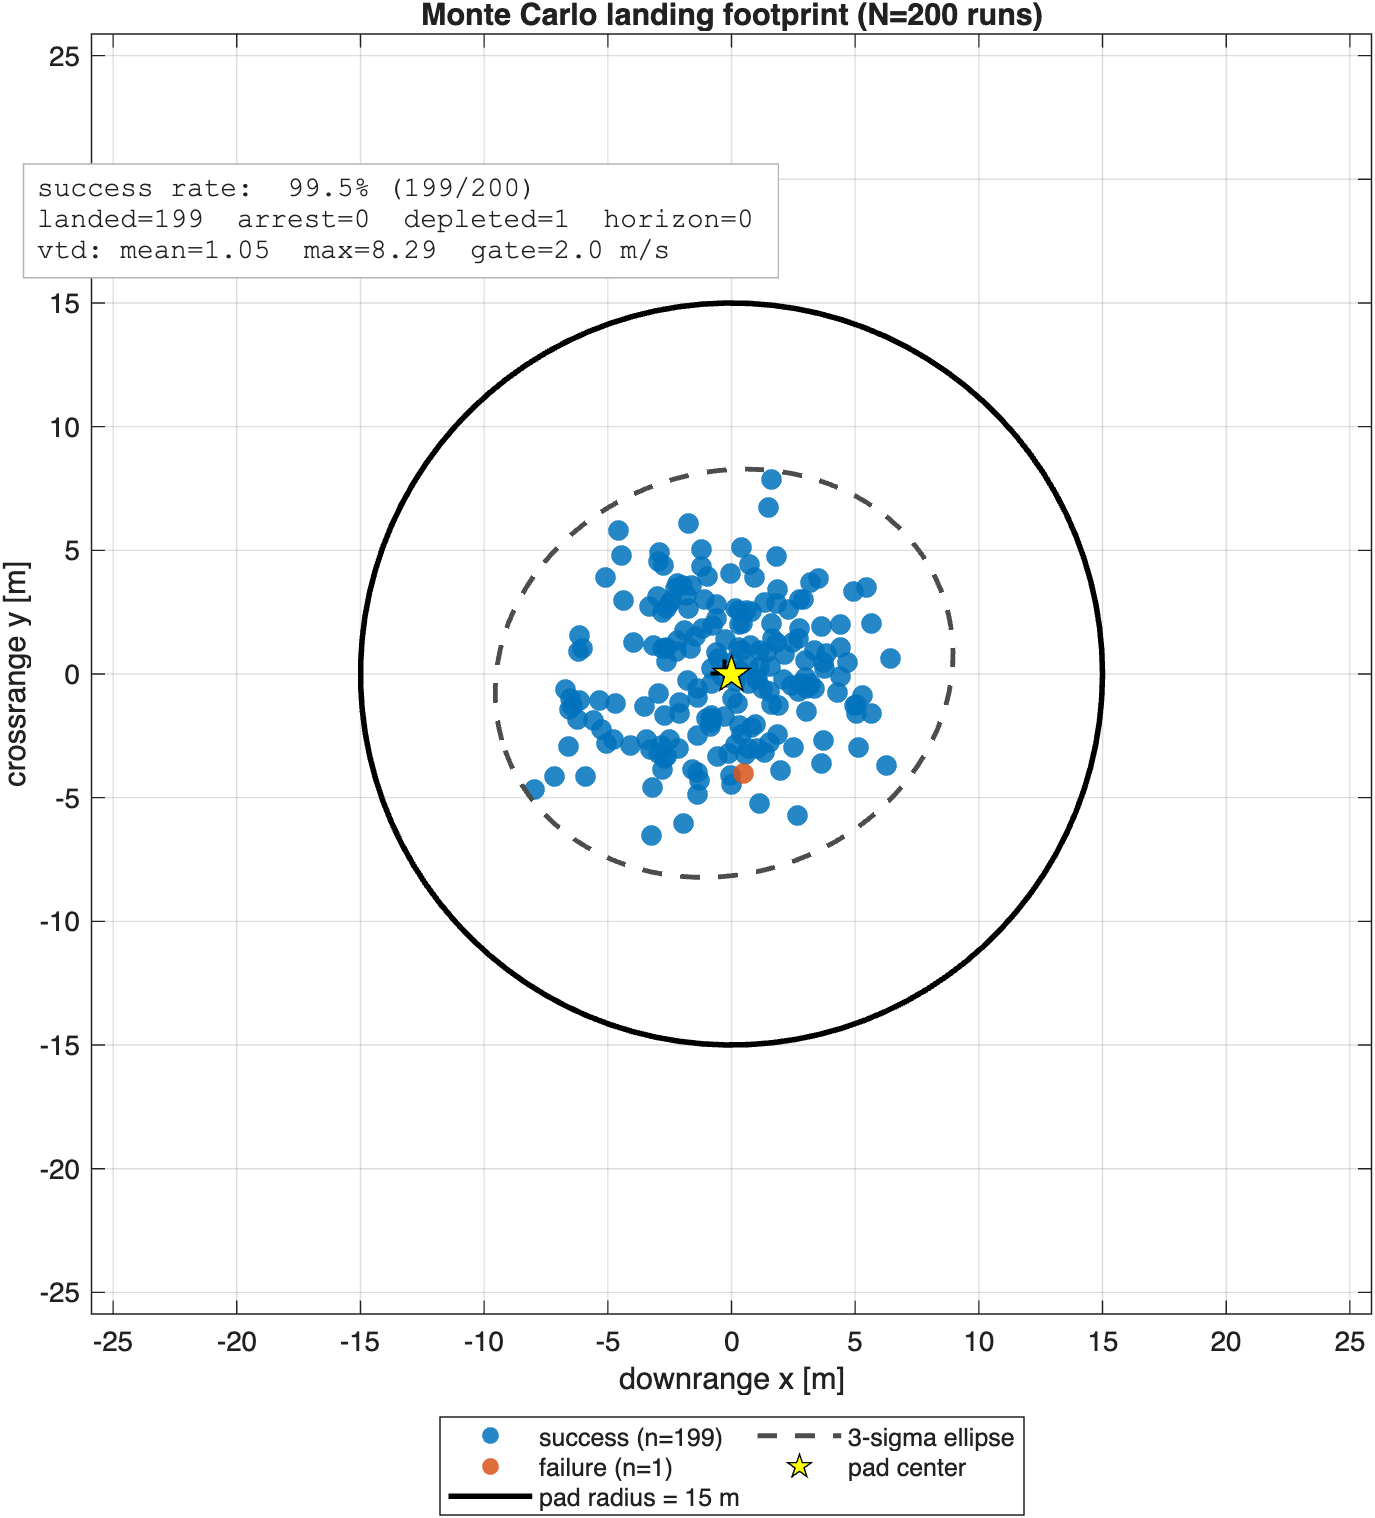
\includegraphics[width=0.62\textwidth]{footprint.png}
\caption{Phase-1 landing footprint, 200 dispersed runs. The dispersion
ellipse is centred on the sample mean (a documented convention) and the
circle is the $R_{pad} = 15$~m accuracy requirement.}
\label{fig:footprint}
\end{figure}

\section{Phase 2: atmosphere and drag}
\label{sec:phase2}

Phase 2 re-solves the identical problem with the exponential-atmosphere drag
term \eqref{eq:drag} active, warm-started from the Phase-1 vacuum solution.
Vacuum remains the certified flagship configuration; Phase 2 is a comparison
campaign layered on top of it, not a replacement.

\subsection{The result, which is counterintuitive}

\begin{table}[htbp]
\centering
\caption{Vacuum versus drag, same grid, same boundary conditions.}
\label{tab:phase2}
\begin{tabular}{lrrr}
\toprule
& vacuum & drag & difference \\
\midrule
$t_f$ [s] & $16.595$ & $17.531$ & $+0.936$ (longer) \\
$m(t_f)$ [kg] & $26464.589$ & $26899.276$ & $+434.687$ \\
propellant used [kg] & $3535.411$ & $3100.724$ & $-434.687$ ($-12.30\%$) \\
switch time [s] & $6.155$ & $10.957$ & $+4.802$ \\
braking arc [s] & $10.440$ & $6.574$ & $-3.866$ \\
altitude at switch [m] & $914.7$ & $378.9$ & $-535.8$ \\
speed at switch [m/s] & $175.4$ & $119.1$ & $-56.3$ \\
\bottomrule
\end{tabular}
\end{table}

Table~\ref{tab:phase2} is the comparison, and Figure~\ref{fig:phase2}
shows it. Drag \emph{saves} $434.7$~kg of propellant --- $12.3\%$ of the vacuum
budget --- while \emph{lengthening} the flight by $0.94$~s. The saving is
unsurprising once stated (the atmosphere brakes for free); the lengthening
looks wrong until the arc structure is examined.

\paragraph{The coast-extension mechanism.}
The extra time is not spread over the flight; it is concentrated in the
minimum-throttle arc. That arc lengthens by $4.80$~s while the braking arc
\emph{shortens} by $3.87$~s, netting $+0.94$~s. Drag decelerates the vehicle
during the $\Tmin$ margin arc at no propellant cost, so the vehicle can
afford to fall for longer and arrive at the braking point slower and lower
--- $119.1$~m/s at $378.9$~m instead of $175.4$~m/s at $914.7$~m. Less
velocity to kill from a lower altitude means a shorter, cheaper burn. Flight
time goes up precisely because the \emph{free} part of the deceleration is
doing more of the work, which is the same trade the min--max argument of
\S\ref{sec:minmax} makes: delay the expensive braking as long as possible.
It is also a direct corroboration of that section --- drag makes the
approach colder, and the switch moves later, exactly as predicted.\footnote{Switch
times here are measured as the mid-annulus crossing of $\lVert\Tvec\rVert$
on the node grid with linear interpolation, the same detector the tracker
uses to place its phase schedule.}

This mechanism was independently reproduced during review with a
hand-built two-arc analytic model that shares no code with the campaign,
agreeing with the solver to better than $1\%$.

\begin{figure}[htbp]
\centering
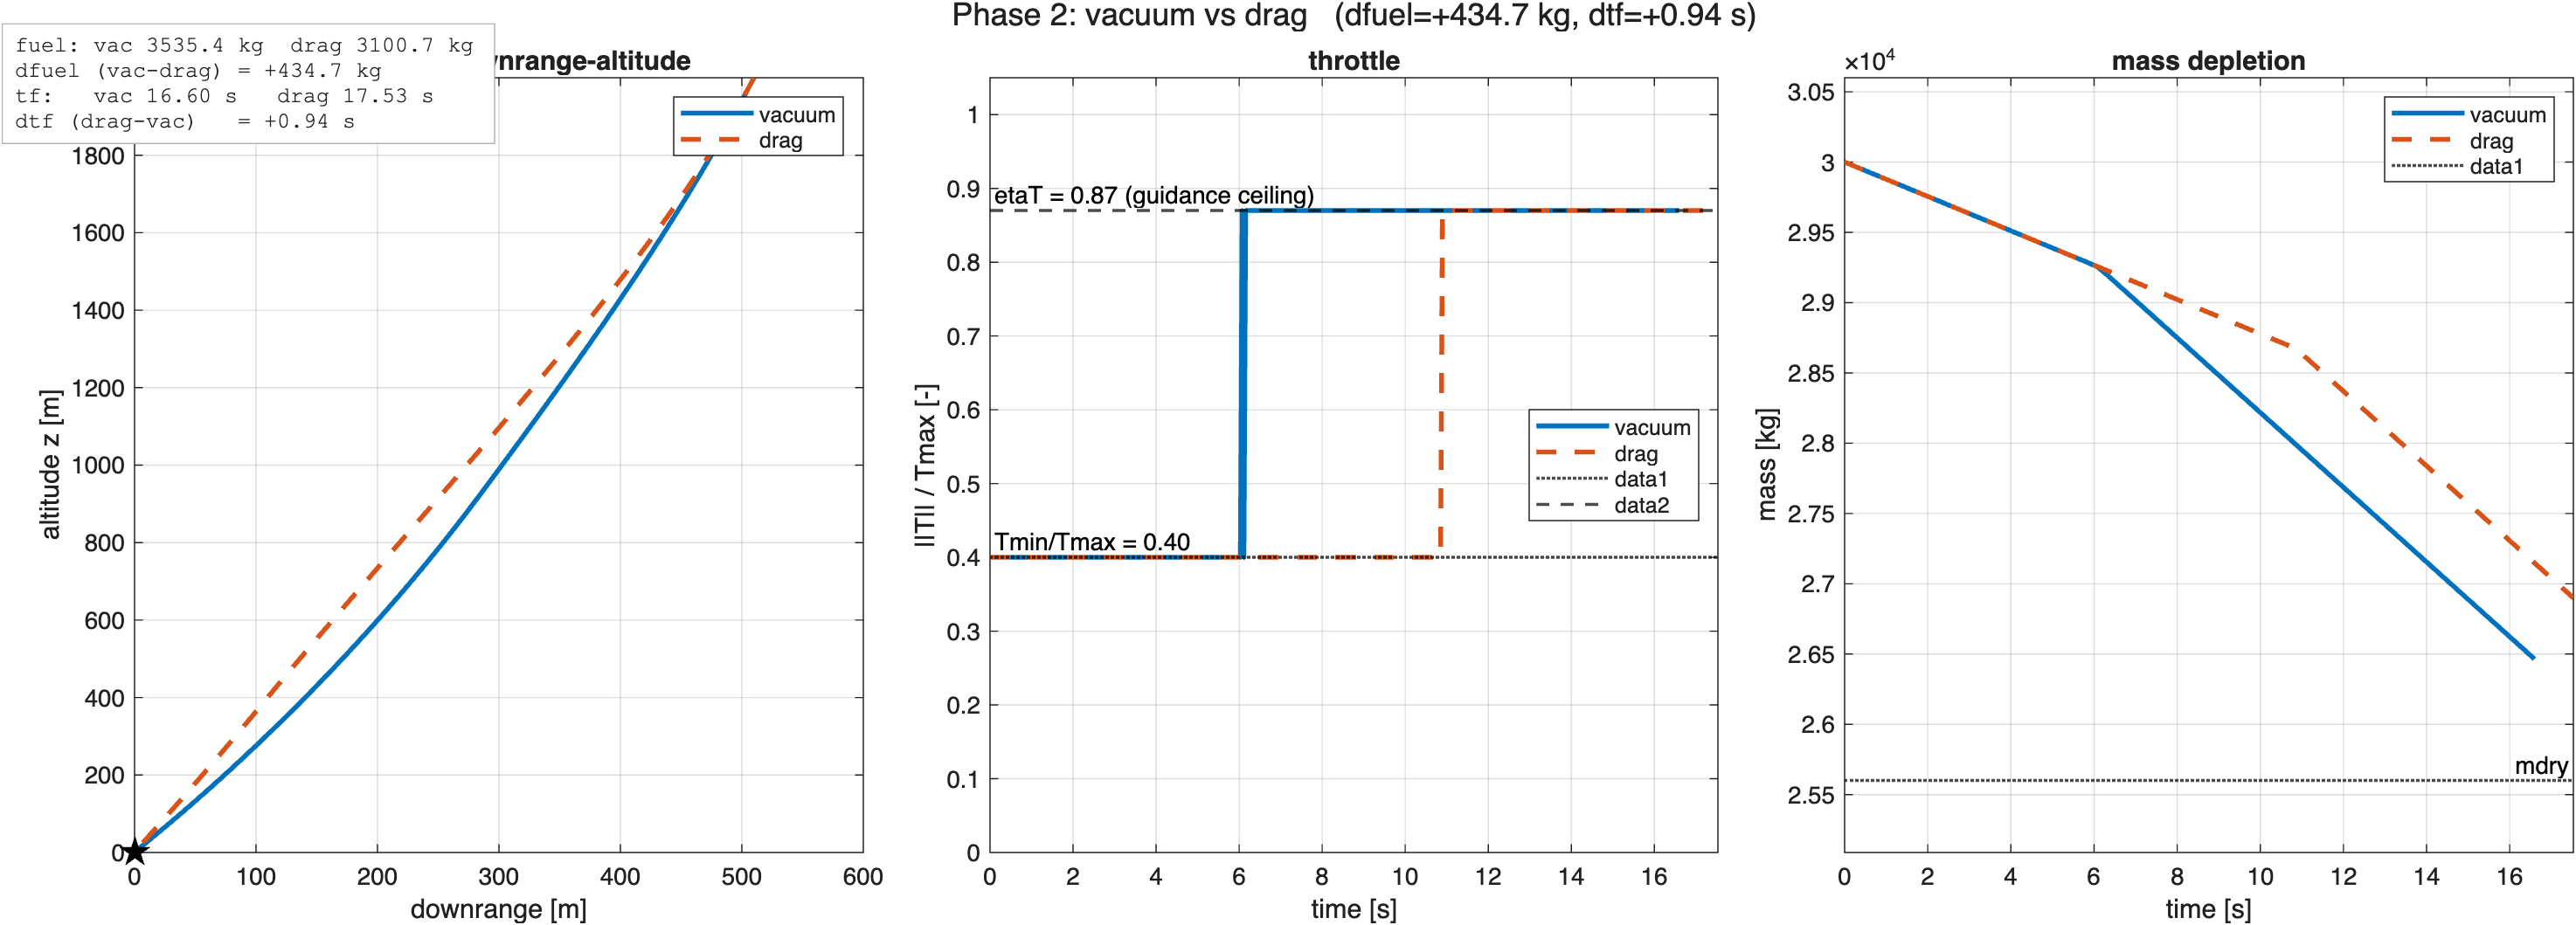
\includegraphics[width=\textwidth]{phase2_vac_vs_drag.png}
\caption{Vacuum versus drag: trajectory, throttle and mass. The throttle
panel shows the mechanism directly --- the minimum-throttle arc extends and
the maximum-throttle braking arc contracts.}
\label{fig:phase2}
\end{figure}

\subsection{What certification can and cannot say under drag}

Gates G1, G2, G2ff and G5 apply unchanged. G3 and G4 are \emph{skipped}, and
the reason is a point of principle rather than convenience: lossless
convexification is exact for the vacuum problem because the change of
variables \eqref{eq:cov} makes those dynamics linear. Drag is quadratic in
velocity and exponential in altitude; there is no convex twin, so there is
nothing to cross-validate against and no relaxation whose tightness could be
measured. Reporting a G3 number under drag would be reporting a fiction.

\begin{center}
{\footnotesize
\begin{tabular}{lrrl}
\toprule
gate & value & threshold & verdict \\
\midrule
G1 max HS defect        & $2.28\times10^{-8}$ & $<10^{-6}$ & PASS \\
G2 pos residual [m]     & $0.0123$ & $<1$ & PASS \\
G2 vel residual [m/s]   & $6.60\times10^{-4}$ & $<0.1$ & PASS \\
G2 mass residual [kg]   & $1.03\times10^{-4}$ & $<0.5$ & PASS \\
G2ff below/above        & $1.7\times10^{-16}$ / $1.6\times10^{-16}$ & $<10^{-6}$ & PASS \\
G3, G4                  & --- & --- & skipped (no convex twin) \\
G5 bound fraction       & $1.000$ & $\ge 0.95$ & PASS \\
G5 interior switches    & $1$ & $\le 2$ & PASS \\
G5 primer angle [deg]   & $2.605$ & $<10$ (loosened) & PASS \\
\bottomrule
\end{tabular}}
\end{center}

Two adaptations are worth recording honestly.

First, G5's primer threshold is \emph{loosened} from $1^\circ$ to $10^\circ$
under drag, not removed. An earlier version of the change did remove it, by
setting the gate to the structure check alone, and review correctly caught
that as a regression risk: with the primer check gone, a sign-flip bug would
silently pass. The loosened threshold sits more than $3\times$ above the
measured $2.605^\circ$ while still catching the $90$--$180^\circ$
misalignments that constitute the real failure mode. The measurement behind
the number: the same coarse grid that gives a vacuum primer angle of
$1.14^\circ$ gives $5.11^\circ$ under drag, and at the production grid
(where vacuum clears $1^\circ$ comfortably) drag still measures
$2.605^\circ$ --- so finer meshing does \emph{not} cure it the way it cures
the vacuum discretization artifact. Analytically the direction condition
should be unchanged by drag: drag enters the dynamics Jacobian $A$ but never
$B = \partial\dot{x}/\partial\Tvec$, so the Hamiltonian's control-dependent
term is untouched and the maximizing direction is still
$+\lamv/\lVert\lamv\rVert$. The most likely explanation is degradation in
how well the discrete defect dual approximates the continuous costate once
the residual's curvature grows under the $\lVert\vvec\rVert\vvec$
nonlinearity. That is an open question, flagged rather than force-closed.

Second, the NLP convergence tolerance is tightened from $10^{-9}$ to
$10^{-11}$ under drag. G1 initially failed at $3.21\times10^{-6}$, entirely
concentrated in the \emph{mass} row of the \emph{first} segment. The cause
was traced, not guessed: IPOPT's own constraint violation at $10^{-9}$ was
$1.07\times10^{-10}$ in nondimensional units, and $1.07\times10^{-10}\times
M_c = 3.21\times10^{-6}$~kg matches the observed defect to five significant
figures. The solver had converged to the tolerance it was asked for; the
$M_c = 30\,000$ unscaling turned an unremarkable nondimensional residual
into an SI defect above an \emph{absolute} SI gate. Deepening convergence
fixes it ($10^{-10} \to 8.87\times10^{-7}$, $10^{-11} \to
2.28\times10^{-8}$) with $m_f$ unchanged to $0.001$~kg across the entire
sweep --- confirming a convergence-depth choice with no physical
consequence. The principled fix is a per-row-scaled G1 tolerance, noted in
\S\ref{sec:future}.

\subsection{Wind Monte Carlo}

\begin{table}[htbp]
\centering
\caption{Phase-2 Monte Carlo, 200 runs, drag active, wind dispersion on.}
\label{tab:mcd}
\begin{tabular}{lr}
\toprule
success rate & $99.0\%$ (198 / 200) \\
failure modes & 0 arrests, 0 horizon expiries, 2 pad-radius misses \\
miss: mean / median / p95 / max & $6.02$ / $5.62$ / $12.38$ / $15.52$ m \\
$v_{td}$: mean / max & $0.919$ / $1.125$ m/s \\
propellant remaining: min / mean & $477.3$ / $994.1$ kg \\
largest wind drawn & $34.7$ m/s \\
\bottomrule
\end{tabular}
\end{table}

Table~\ref{tab:mcd} and Figure~\ref{fig:phase2footprint} give the result.
The Phase-2 failure population is qualitatively different and, from a safety
standpoint, better: \textbf{every one of the 200 runs achieved a genuine
touchdown}, and the two failures are pad-radius misses at $15.52$~m and
$15.15$~m against a $15$~m requirement --- a $3\%$ and $1\%$ overshoot of an
accuracy requirement, not a loss of vehicle. No run exceeded $1.13$~m/s at
contact, and the worst run still had $477$~kg of propellant left. The wider
footprint is the wind: the worst miss (run 43, $15.52$~m) drew
$\mathbf{w} = [25.74;\ -9.41;\ 0]$~m/s, a $27.4$~m/s steady wind, which
pushes the vehicle farther than the fixed-reference tracker fully recovers
within the burn.

\begin{figure}[htbp]
\centering
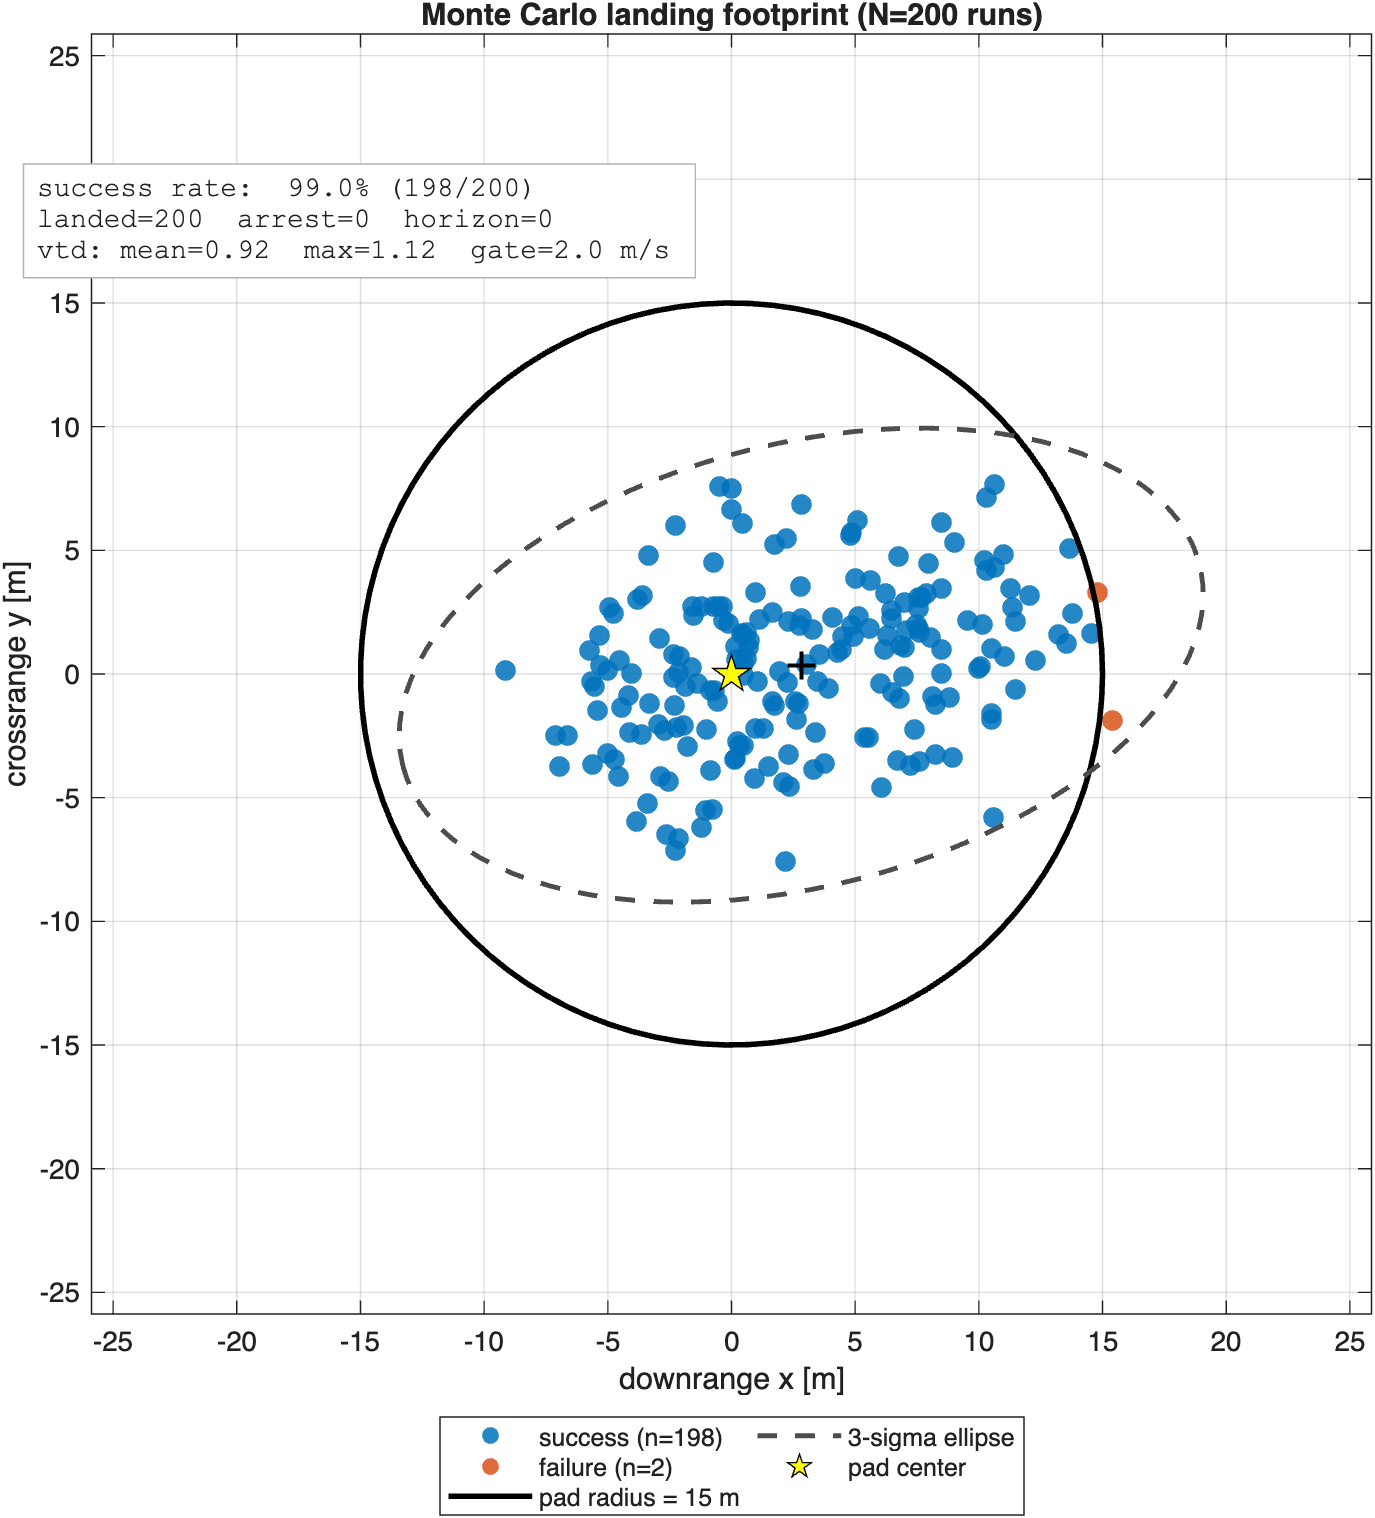
\includegraphics[width=0.62\textwidth]{phase2_footprint.png}
\caption{Phase-2 landing footprint, 200 runs with drag and wind. Compare
Figure~\ref{fig:footprint}: the distribution is wider and biased downwind,
but the tail is a miss-distance tail rather than a touchdown-speed tail.}
\label{fig:phase2footprint}
\end{figure}

\section{Future work}
\label{sec:future}

\begin{itemize}

\item \textbf{Six degrees of freedom.} The current model is a point mass
with an instantaneously steerable thrust vector. A 6-DOF model with
attitude dynamics and a finite gimbal rate would put a real bandwidth limit
on the direction channel, which is exactly the channel
\S\ref{sec:pole} showed the controller leaning on hardest during the margin
arc. The pointing cone constraint is already implemented and disabled;
enabling it is the natural first step. One certification wrinkle is already
handled: Gate~G5's primer-vector sub-check (thrust parallel to the velocity
costate) is a necessary condition only for the \emph{unconstrained} problem,
and is invalid once the cone is active --- with a finite cone the optimal
thrust rides the cone boundary (the projection of the unconstrained
direction onto it), so thrust need not be parallel to the costate by
design, not by bug. \texttt{certify\_pdg.m} is cone-aware: when
\texttt{P.theta\_max\_deg} is finite the primer angle is still computed and
reported but only as information (\texttt{G5\_primer\_mode =
'skipped-cone'}), and G5's pass/fail rests on the bang-bang structure check
alone.

\item \textbf{The full return profile.} This campaign begins at the
post-entry-burn state. Entry burn, aerodynamic descent with grid fins, and
the handover to the landing burn are all upstream, and the handover state is
currently an assumption rather than a result.

\item \textbf{Successive convexification (SCvx).} Phase 2 loses G3 and G4
because drag has no lossless convex twin. SCvx~\cite{mao2016} would restore
a convex-solver route for the drag problem by linearizing the nonconvex
dynamics about a reference and iterating with a trust region, which would
give Phase~2 back a genuine cross-method check --- currently its most
significant certification gap.

\item \textbf{A real conic solver.} The convex subproblems are
currently solved with IPOPT, a general nonlinear interior-point method.
They are SOCPs; a dedicated conic solver such as ECOS~\cite{ecos2013} is a
documented drop-in and would be both faster and better conditioned. It was
deliberately not made a dependency for this campaign.

\item \textbf{Model-predictive guidance and replanning.} This is the
most important item, and \S\ref{sec:derate} is the argument for it. The
$82.30$~kg de-rate exists solely because \emph{a fixed-reference tracker
cannot re-time the brake}: the reachability table shows a $-5\%$ vehicle
must brake $107$~m higher, and no feedback gain around a fixed feed-forward
can do that. A guidance law that re-solves the PDG problem in flight ---
even coarsely, even a few times --- \emph{can}, and would recover most of
the de-rate's propellant cost while improving robustness rather than
trading against it. The solve times measured here (well under a second at
$N = 60$) suggest this is within reach.

\item \textbf{Per-row scaled G1 tolerance.} Phase 2 exposed that G1's
absolute SI threshold implicitly weights the mass row by $M_c = 30\,000$
relative to the nondimensional residual IPOPT actually controls. The
workaround --- deepen convergence --- is measured and harmless, but the
principled fix is to scale the G1 tolerance per state row by that row's own
characteristic magnitude.

\item \textbf{The drag primer question.} \S\ref{sec:phase2} leaves open why
the discrete defect duals approximate the continuous costate less well under
drag when the direction condition is analytically drag-independent. A grid
refinement study run to convergence would settle it.

\end{itemize}

\section*{Reproduction}

The whole campaign is one call from a fresh MATLAB session:

{\footnotesize
\begin{verbatim}
/Applications/MATLAB_R2025b.app/bin/matlab -batch \
  "cd('<repo>/booster_landing'); run_booster_landing"
\end{verbatim}
}

\begin{sloppypar}
\noindent
which solves both routes, certifies, designs the tracker, runs the
Monte Carlo, and writes \texttt{booster\_run.mat} into \texttt{results/},
along with the figures
reproduced in this note. Passing the option \texttt{phase2 = true} adds the
Phase-2 stage. Every number quoted here was read from that file. All
parameters are overridable through an optional \texttt{cfg} struct without
editing a library file.
\end{sloppypar}

\begin{thebibliography}{99}

\bibitem{acikmese2007}
Ac\i kme\c{s}e, B., and Ploen, S.~R.,
``Convex Programming Approach to Powered Descent Guidance for Mars
Landing,''
\emph{Journal of Guidance, Control, and Dynamics}, Vol.~30, No.~5, 2007,
pp.~1353--1366.

\bibitem{blackmore2010}
Blackmore, L., Ac\i kme\c{s}e, B., and Scharf, D.~P.,
``Minimum-Landing-Error Powered-Descent Guidance for Mars Landing Using
Convex Optimization,''
\emph{Journal of Guidance, Control, and Dynamics}, Vol.~33, No.~4, 2010,
pp.~1161--1171.

\bibitem{acikmese2011}
Ac\i kme\c{s}e, B., and Blackmore, L.,
``Lossless Convexification of a Class of Optimal Control Problems with
Non-Convex Control Constraints,''
\emph{Automatica}, Vol.~47, No.~2, 2011, pp.~341--347.

\bibitem{kelly2017}
Kelly, M.,
``An Introduction to Trajectory Optimization: How to Do Your Own Direct
Collocation,''
\emph{SIAM Review}, Vol.~59, No.~4, 2017, pp.~849--904.

\bibitem{betts2010}
Betts, J.~T.,
\emph{Practical Methods for Optimal Control and Estimation Using Nonlinear
Programming}, 2nd ed., SIAM, Philadelphia, 2010.

\bibitem{anderson1990}
Anderson, B.~D.~O., and Moore, J.~B.,
\emph{Optimal Control: Linear Quadratic Methods}, Prentice-Hall,
Englewood Cliffs, NJ, 1990.

\bibitem{lawden1963}
Lawden, D.~F.,
\emph{Optimal Trajectories for Space Navigation}, Butterworths, London,
1963.

\bibitem{ipopt2006}
W\"achter, A., and Biegler, L.~T.,
``On the Implementation of an Interior-Point Filter Line-Search Algorithm
for Large-Scale Nonlinear Programming,''
\emph{Mathematical Programming}, Vol.~106, No.~1, 2006, pp.~25--57.

\bibitem{casadi2019}
Andersson, J.~A.~E., Gillis, J., Horn, G., Rawlings, J.~B., and Diehl, M.,
``CasADi: A Software Framework for Nonlinear Optimization and Optimal
Control,''
\emph{Mathematical Programming Computation}, Vol.~11, No.~1, 2019,
pp.~1--36.

\bibitem{mao2016}
Mao, Y., Szmuk, M., and Ac\i kme\c{s}e, B.,
``Successive Convexification of Non-Convex Optimal Control Problems and Its
Convergence Properties,''
\emph{Proceedings of the 55th IEEE Conference on Decision and Control},
Las Vegas, NV, 2016, pp.~3636--3641.

\bibitem{ecos2013}
Domahidi, A., Chu, E., and Boyd, S.,
``ECOS: An SOCP Solver for Embedded Systems,''
\emph{Proceedings of the European Control Conference}, Z\"urich, 2013,
pp.~3071--3076.

\bibitem{boyd2004}
Boyd, S., and Vandenberghe, L.,
\emph{Convex Optimization}, Cambridge University Press, Cambridge, 2004.

\end{thebibliography}

\end{document}
